%%% Local Variables:
%%% mode: latex
%%% TeX-master: t
%%% End:

%\documentclass[doctor,secret]{ucasthesis}
\documentclass[master, secret]{ucasthesis}
%\documentclass[doctor]{ucasthesis}
% \documentclass[%
%   master|doctor, % mandatory option
%   secret,
%   arialtoc,arialtitle]{ucasthesis}

% 所有其他可能用到的包都统一放到这里了,可以根据自己的实际添加或者删除。
\usepackage{ucastils}

\usepackage{booktabs}% http://ctan.org/pkg/booktabs
\newcommand{\tabitem}{~~\llap{\textbullet}~~}


\usepackage{supertabular} %跨页表格
\usepackage{colortbl} %彩色表格宏包
\usepackage{tablefootnote}

\usepackage{longtable}
\usepackage{array} % for extrarowheight
\setlength{\extrarowheight}{1.5pt}

%伪代码
\usepackage{algorithm}
\usepackage{algpseudocode,float}
\usepackage{amsmath}

\floatname{algorithm}{算法}
\renewcommand{\algorithmicrequire}{\textbf{输入:}}
\renewcommand{\algorithmicensure}{\textbf{输出:}}

\makeatletter
\newenvironment{breakablealgorithm}
  {% \begin{breakablealgorithm}
   \begin{center}
     \refstepcounter{algorithm}% New algorithm
     \hrule height.8pt depth0pt \kern2pt% \@fs@pre for \@fs@ruled
     \renewcommand{\caption}[2][\relax]{% Make a new \caption
       {\raggedright\textbf{\ALG@name~\thealgorithm} ##2\par}%
       \ifx\relax##1\relax % #1 is \relax
         \addcontentsline{loa}{algorithm}{\protect\numberline{\thealgorithm}##2}%
       \else % #1 is not \relax
         \addcontentsline{loa}{algorithm}{\protect\numberline{\thealgorithm}##1}%
       \fi
       \kern2pt\hrule\kern2pt
     }
  }{% \end{breakablealgorithm}
     \kern2pt\hrule\relax% \@fs@post for \@fs@ruled
   \end{center}
  }
\makeatother

%代码
\usepackage{listings}
\lstset{
  language=[ANSI]c,
  basicstyle=\small,
  numbers=left,
  keywordstyle=\color{blue},
  numberstyle={\tiny\color{lightgray}},
  stepnumber=1, %行号会逐行往上递增
  numbersep=5pt,
  commentstyle=\small\color[rgb]{0.5,0.5,0.5},
  backgroundcolor=\color[rgb]{0.95,1.0,1.0},
  showspaces=false,
  showtabs=false,
  frame=shadowbox, framexleftmargin=5mm, rulesepcolor=\color{red!20!green!20!blue!20!},
% frame=single,
%  TABframe=single,
  tabsize=4,
  breaklines=tr,
  extendedchars=false %这一条命令可以解决代码跨页时,章节标题,页眉等汉字不显示的问题
}

% figure left, right
\usepackage[export]{adjustbox}

% 你可以在这里修改配置文件中的定义,导言区可以使用中文。
% \def\myname{胡庆海}

\begin{document}

% 定义所有的eps文件在 figures 子目录下
\graphicspath{{figures/}}

%%% 封面部分
\frontmatter

%%% Local Variables:
%%% mode: latex
%%% TeX-master: t
%%% End:
\secretcontent{绝密}

\ctitle{龙芯平台下Mesa3D图形库的性能优化}
% 根据自己的情况选,不用这样复杂
\makeatletter

\makeatother

\cdegree{工程硕士}
\cdepartment[计算所]{中国科学院计算技术研究所}
\cmajor{计算机技术}
\cauthor{胡庆海} 
\csupervisor{胡伟武\hspace{1em}研究员}
\csupervisorplace{中国科学院计算技术研究所}
% 如果没有副指导老师或者联合指导老师,把下面两行相应的删除即可。


% 日期自动生成,如果你要自己写就改这个cdate
%\cdate{\CJKdigits{\the\year}年\CJKnumber{\the\month}月}

% 博士后部分
% \cfirstdiscipline{计算机科学与技术}
% \cseconddiscipline{系统结构}
% \postdoctordate{2009年7月——2011年7月}

\etitle{Performance Optimization of Mesa3D Graphics Library on Loongson Platform}
% 这块比较复杂,需要分情况讨论:
% 1. 学术型硕士
%    \edegree:必须为Master of Arts或Master of Science(注意大小写)
%              “哲学、文学、历史学、法学、教育学、艺术学门类,公共管理学科
%               填写Master of Arts,其它填写Master of Science”
%    \emajor:“获得一级学科授权的学科填写一级学科名称,其它填写二级学科名称”
% 2. 学术型博士
%    \edegree:Doctor of Philosophy(注意大小写)
%    \emajor:“获得一级学科授权的学科填写一级学科名称,其它填写二级学科名称”

\edegree{Master of Computer Architecture}
\eauthor{Hu Qinghai}
\edepartment{Institute of Computing Technology\\Chinese Academy of Sciences}
\emajor{Computer Technology}
\esupervisor{Hu Weiwu}

% 这个日期也会自动生成,你要改么?
% \edate{December, 2005}

% 定义中英文摘要和关键字
\begin{cabstract}

  OpenGL是行业领域中最为广泛接纳的2D/3D图形API, 其自诞生至今已催生了各种计算机平台及设备上的数千优秀应用程序。而随着龙芯CPU的产业化加速,基于OpenGL的图形应用程序越来越多,于是在龙芯平台上广泛使用的OpenGL的一种开源实现Mesa图形库的性能就是决定龙芯平台的客户使用体验的重中之重。本文则是针对Mesa图形库的性能优化展开的相关工作。

  本文完成的主要工作和贡献如下:

  第一,显示列表

  第二,内存到显存的优化

  第三,热点代码优化

  在龙芯软硬件平台上对本文提出的优化方案进行了效果验证和测试。其中显示列表优化效果...内存到显存优化效果...热点代码优化效果...。本文优化成果已经集成到龙芯Mesa图形库应用产品中。

\end{cabstract}

\ckeywords{Mesa, OpenGL, MIPS, GPU, 龙芯, 性能优化}

\begin{eabstract} 
   An abstract of a dissertation is a summary and extraction of research work
   and contributions. Included in an abstract should be description of research
   topic and research objective, brief introduction to methodology and research
   process, and summarization of conclusion and contributions of the
   research. An abstract should be characterized by independence and clarity and
   carry identical information with the dissertation. It should be such that the
   general idea and major contributions of the dissertation are conveyed without
   reading the dissertation. 

   An abstract should be concise and to the point. It is a misunderstanding to
   make an abstract an outline of the dissertation and words ``the first
   chapter'', ``the second chapter'' and the like should be avoided in the
   abstract.

   Key words are terms used in a dissertation for indexing, reflecting core
   information of the dissertation. An abstract may contain a maximum of 5 key
   words, with semi-colons used in between to separate one another.
\end{eabstract}

\ekeywords{Mesa, OpenGL, MIPS, GPU, Loongson, Performance Optimization}

% 设置 PDF 文档的作者、主题等属性
\makeatletter
\ucas@setup@pdfinfo
\makeatother
\makecover

% 目录
\tableofcontents
% 插图索引
\listoffigures
% 表格索引
\listoftables
% 符号对照表
\begin{denotation}

\item[API] 应用程序编程接口 (Application Programming Interface)
\item[CPU] 中央处理器 (Central Processing Unit)
\item[GPU] 图形处理器 (Graphics Processing Unit)
\item[HPC] 高性能计算 (High Performance Computing)
\end{denotation}


%%% 正文部分
\mainmatter

%%% Local Variables:
%%% mode: latex
%%% TeX-master: t
%%% End:

\chapter{引言}
\label{cha:intro}
  
\section{研究背景}

\subsection{Linux图形系统体系栈}
\subsubsection{早期Linux下的2D图形体系栈}
在早期,Linux下的应用程序的绘制都不是直接绘制,而是通过X-Server来进行绘制。应用程序通过Xlib库并遵守X11协议向X-Server发送渲染指令,然后X-Server接受这些指令并处理和转化为硬件指令,并将这些硬件指令发送给GPU让其执行。具体流程如图\ref{fig:2D-Graph-Stack}所示

\begin{figure}[H] 
  \centering
  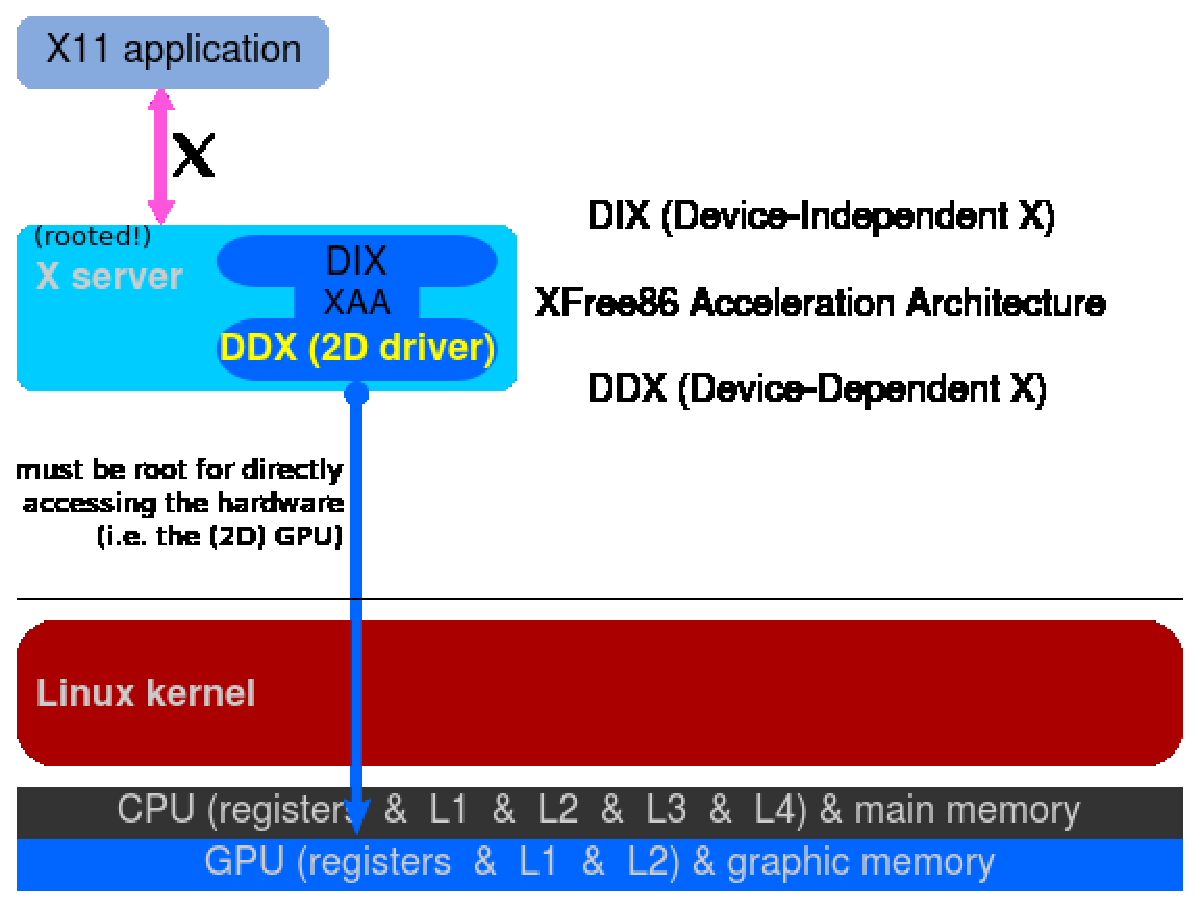
\includegraphics[width=10cm,height=6cm]{figures/chap01/Linux_graphics_drivers_2D}
  \caption{早期Linux下2D图形系统体系栈}
  \label{fig:2D-Graph-Stack}
\end{figure}

\subsubsection{支持3D图形渲染的Linux图形体系栈}
经过不断的发展,Linux通过OpenGL实现了3D图形渲染,其中3D图形渲染的方法主要有两种:
\begin{itemize}
\item{\textbf{Indirect Rendering}}: \\
在一些传统的系统平台上,由于只能唯一通过X-Server访问图形硬件,所以只能向X-Server发送绘制指令然后再通过X-Server转化为硬件命令给GPU执行,这种方式和传统的2D绘制方式相似。
\item{\textbf{Direct Rendering}}: \\ 
随着系统平台上的发展,直接渲染框架(Direct Rendering Infrastructure)的诞生使得OpenGL程序可以通过Linux内核的drm库直接与图形硬件(GPU)进行交互,这一进步极大的提高了3D渲染的效率,成为当今比较主流的渲染方式。
\end{itemize}

\begin{figure}[H] 
  \centering
  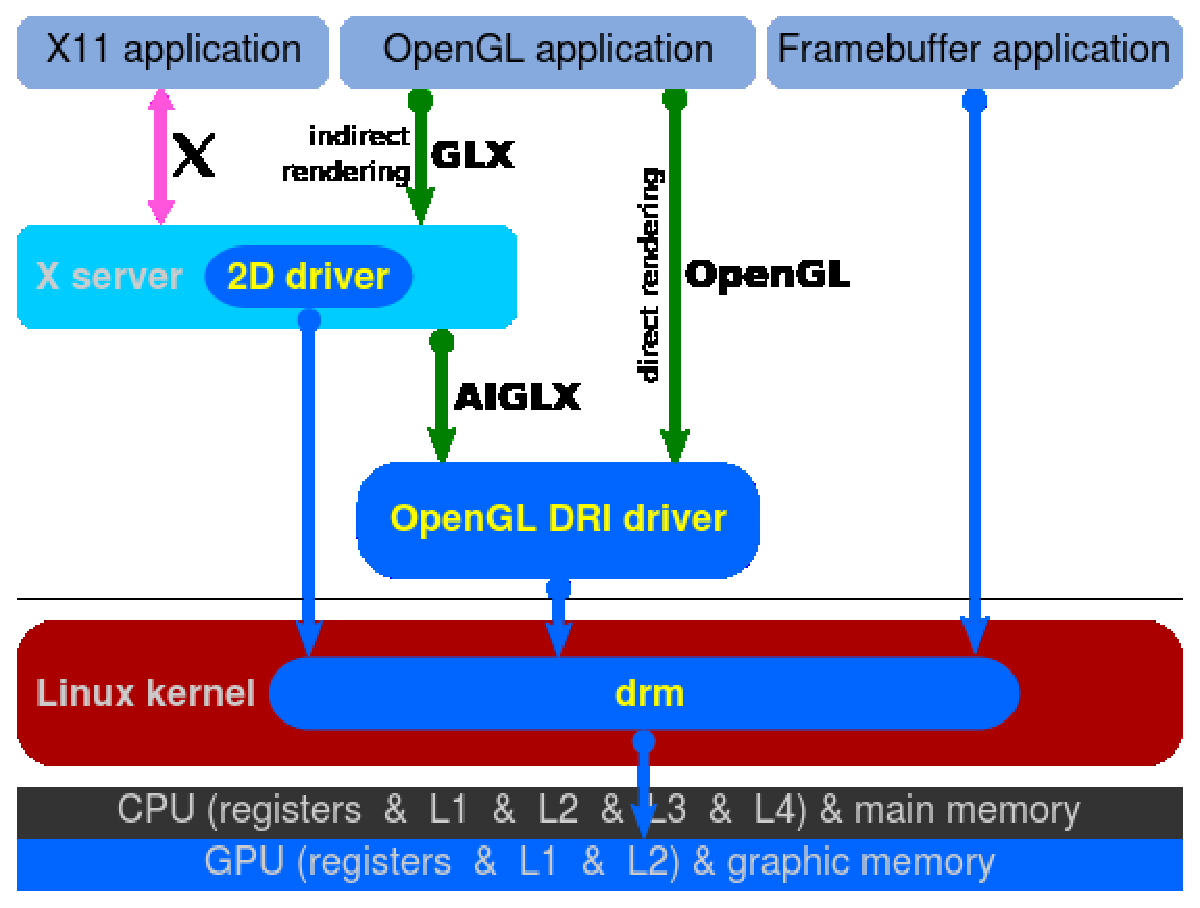
\includegraphics[width=10cm,height=6cm]{figures/chap01/OpenGL_With_Direct_Rendering}
  \caption{Linux下3D图形系统体系栈}
  \label{fig:OpenGL_With_Direct_Rendering}
\end{figure}



\subsection{OpenGL}

\subsubsection{OpenGL基本介绍}
开放图形库(Open Graphics Library,缩写为OpenGL)是个定义了一个跨编程语言、跨平台的应用程序接口(API)的规范,它用于生成2D、3D图像。这个接口由近350个不同的函数调用组成,用来从简单的图形比特绘制复杂的三维景象。而另一种程序接口系统是仅用于Microsoft Windows上的Direct3D。OpenGL常用于CAD、虚拟实境、科学可视化程序和电子游戏开发。

OpenGL规范描述了绘制2D和3D图形的抽象API。尽管这些API可以完全通过软件实现,但它是为大部分或者全部使用硬件加速而设计的。OpenGL不仅语言无关,而且平台无关。规范只字未提获得和管理OpenGL上下文相关的内容,而是将这些作为细节交给底层的窗口系统。出于同样的原因,OpenGL纯粹专注于渲染,而不提供输入、音频以及窗口相关的API。

\subsubsection{OpenGL渲染管线}

绝大多数OpenGL实现都有着相似的操作,一系列相关的处理阶段叫做OpenGL渲染管线。图\ref{fig:OpenGL-Pipeline}显示了这些顺序,几何数据(顶点、直线和多边形)所经历的处理阶段包括求值器和基于顶点的操作,而像素数据(像素、图像和位图)的处理过程则有所不同。在最终的像素数据写入到帧缓存之前,这两种类型的数据都经过相同的最终步骤(光栅化和基于片段的操作)\cite{OpenGL-Programming-Guide}。

\begin{figure}[H] 
  \centering
  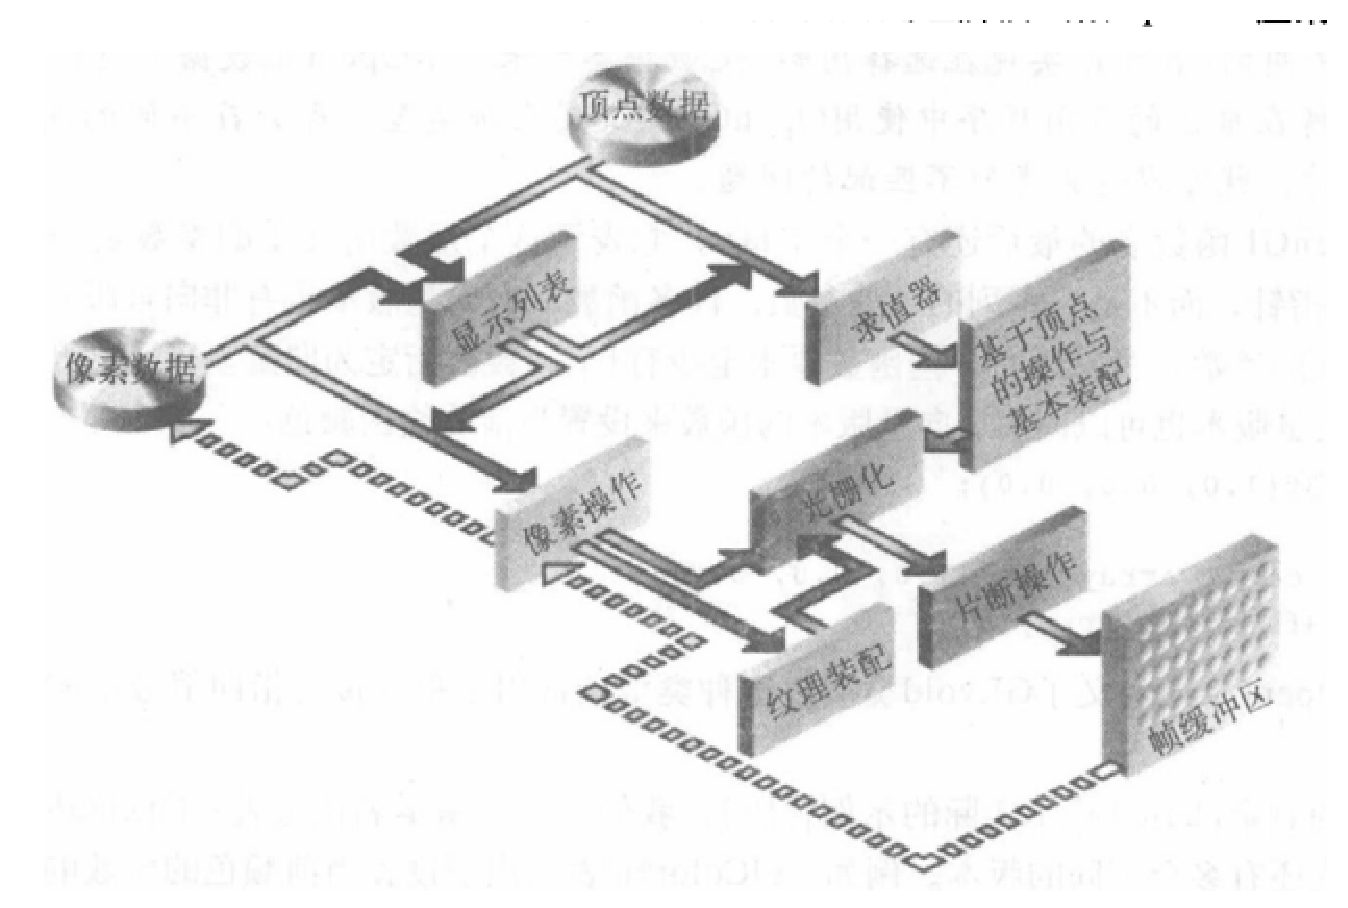
\includegraphics[width=10cm,height=7cm]{figures/chap01/OpenGL-Pipeline}
  \caption{OpenGL渲染管线}
  \label{fig:OpenGL-Pipeline}
\end{figure}

这里详细介绍一下渲染管线上的几个阶段:
\begin{itemize}
\item{\textbf{显示列表}}:\quad几何图形和像素都可以保存到显示列表中,以供当前或者以后使用。当一个显示列表被执行时候,保存的数据就从显示列表取出,就像在立即模式下直接由应用程序发送的那样。
\item{\textbf{求值器}}:\quad所有的几何图形都最终要通过顶点来表示。求值器提供了一种方法,它根据曲线或者表面的控制顶点计算表示曲线或者表面的顶点。这种方法是一种多项式映射,它可以根据控制点产生表面法线,纹理坐标等。
\item{\textbf{基于顶点的操作与图元装配}}:\quad这其实是两个过程,首先基于顶点的操作是把顶点转化为图元,即将空间坐标从3D世界的一个位置投影到屏幕的一个位置。其次图元装配阶段主要内容就是裁剪,它的任务是消除位于某个特定平面以外的部分几何图元。
\item{\textbf{像素操作}}:\quad通常需要对来自系统内存的一个数组中的像素进行解包,接着这些像素数据会被执行像素转化(缩放、偏移、映射和截取)操作。
\item{\textbf{纹理装配}}:\quad OpenGL应用程序可以在几何物体上应用纹理图像,此阶段就是纹理相关的装配处理。
\item{\textbf{光栅化}}:\quad把几何数据和像素数据转化为片段的过程。每个片段对应于帧缓存的一个像素。这个过程会考虑直线的宽度,点的大小,着色模型以及抗锯齿等计算。
\item{\textbf{片段操作}}:\quad数据实际存储到帧缓存区前,还需要执行的一系列操作,比如可能的纹理操作,前面纹理装配阶段产生的纹理内存会为每个片段生成一个纹理单元并与该片段融合。
\end{itemize}

\subsubsection{OpenGL版本变化}
OpenGL是一个不断进化的API。新版OpenGL规范会定期由Khronos Group发布,新版本通过扩展API来支持各种新功能。每个版本的细节由Khronos Group的成员一致决定,包括显卡厂商、操作系统设计人员以及类似Mozilla和谷歌的一般性技术公司。详细历史版本更新参阅附录\ref{cha:OpenGL-History-Version}。



\section{Mesa3D介绍}

\subsection{Mesa3D简介}
Mesa3D最早是由Brian Paul在1993年8月开始开发的一个实现了OpenGL API的开源图形库\cite{Mesa-Wiki}。它目前隶属于freedesktop.org,广泛运用在Liunx, BSD等操作系统。早期的Mesa3D的图形渲染实现是采用纯软件计算实现的,后来随着图形硬件的飞速发展,Mesa3D则转为使用图形硬件进行加速渲染,它广泛支持目前主流的各种图形硬件设备:
\begin{itemize}
\item{}Intel i965,i945,i915
\item{}AMD Radeon series(r200,r300,r600 etc)
\item{}NVIDIA GPUs
\end{itemize}
Mesa3D不仅支持基本的OpenGL API,而还支持OpenGL ES、OpenVG、OpenCL、VDPAU和EGL等。

\begin{figure}[H] 
  \centering
  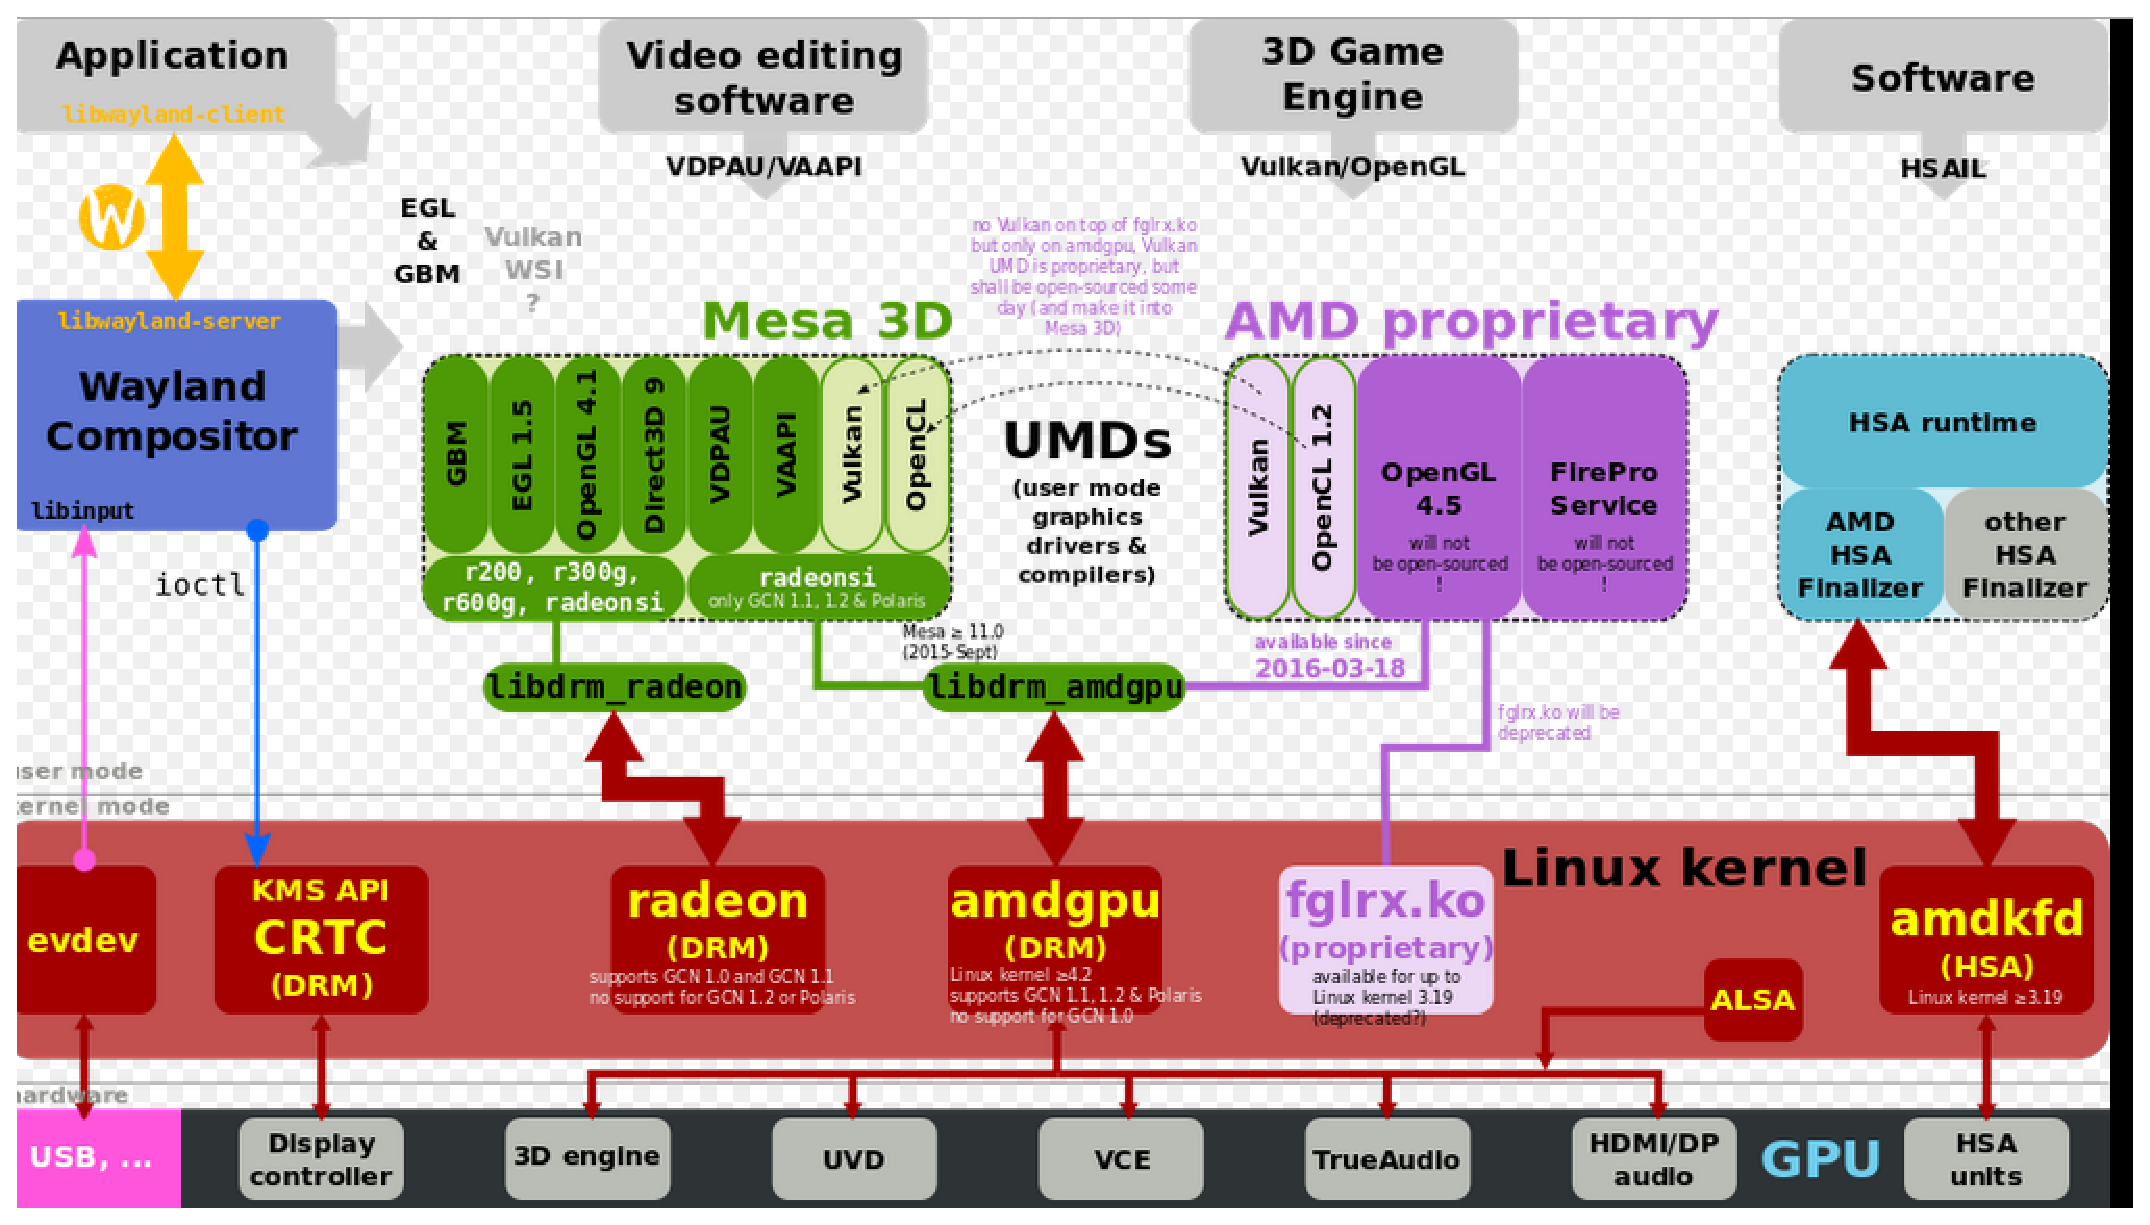
\includegraphics[width=14cm,height=9cm]{figures/chap01/linux-mesa}
  \caption{现代Linux图形栈与Mesa3D}
  \label{fig:linux-mesa}
\end{figure}

\subsection{Mesa3D版本信息}
为了匹配OpenGL的版本不断变化以及各大图形硬件厂商的图形设备不断更新,Mesa3D也一直不断的更新新的版本。到目前为止最新的Mesa3D版本为2016年3月更新的Version 11.2,详细版本更新信息以及支持的OpenGL版本见附录\ref{cha:Mesa3D-History-Version}


\section{龙芯系列处理器介绍}


龙芯处理器主要包括三个系列。龙芯1号处理器及其IP系列主要面向嵌入式应用,龙芯2号超标量处理器及其IP系列主要面向桌面应用,龙芯3号多核处理器系列主要面向服务器和高性能机应用。根据应用的需要,其中部分龙芯2号也可以面向部分高端嵌入式应用,部分低端龙芯3号也可以面向部分桌面应用。以后上述三个系列将并行地发展。

龙芯系列处理器通过充分开发指令级并行性、数据级并行性、线程级并行性来提高性能。其中龙芯1号系列微处理器实现了带有静态分支预测和阻塞Cache的单发射乱序执行流水线;龙芯2号系列微处理器实现了带有动态分支预测和非阻塞Cache的超标量四发射乱序执行流水线,以及还使用浮点数据通路复用技术实现了定点的单指令流多数据流指令;龙芯3号基于可伸缩的多核互连架构设计,在单个芯片上集成多个高性能处理器核以及大量的2级Cache,还通过高速I/O接口实现多芯片的互连以组成更大规模的系统。


\section{本文主要贡献}

本文的主要工作内容如下:

\begin{itemize}
\item{\textbf{立即模式(Immediate Mode)\footnote{OpenGL传统的使用glBegin...glEnd方式制定绘制方式,在这两个函数对之间给出绘制的数据,这种方式称为立即模式。}下顶点数据传输过程研究与优化}}: \\
OpenGL的立即模式下,glBegin与glEnd之间的数据会逐次拷贝到顶点缓冲区中,每当顶点缓存去装载满数据后,这些数据会被传输到图形硬件设备(GPU)显存中,然后再继续装载未装载的数据。本文通过分析这个装载过程的性能瓶颈,提出了一种
\item{\textbf{显示列表(Display List)\footnote{OpenGL显示列表是由一组预先存储起来的留待以后调用的OpenGL函数语句组成的,当调用这张显示列表时就依次执行表中所列出的函数语句。}下CPU与GPU负载平衡的优化}}: \\
通过跟踪分析Mesa3D库代码发现在创建显示列表时候,会先预分配一块缓冲区,当数据溢出时会继续分配一块相同大小的缓冲区,重复此过程直到所有数据都存放到缓冲区中然后提交到显存设备中。这样在面临显示列表中包含大量顶点数据时,就需要分配很多次缓存区,这其中涉及到的数据准备和状态管理等操作都需要GPU来做,这便会导致CPU与GPU的工作负载不平衡,形成性能瓶颈。本文通过根据显示列表数据规模确定缓存区大小的优化方法来解决显示列表的性能瓶颈。
\item{\textbf{内存向显存数据传输优化}}: \\
由于Mesa3D中的顶点数据,属性数据等等都需要传输到显存中,所以内存到显存的数据传输效率就显得至关重要。本文研究分析了现有Mesa3D库内存到显存的数据传输过程,提出了一种简化的数据传输拷贝方式,提高了数据传输速度。
\end{itemize}



本文的研究工作均在龙芯3A系列软硬件平台上使用主流OpenGL性能测试集svPerfGL\footnote{svPerfGL是一个开源的OpenGL基准测试集合,它主要用来测量科学可视化应用的真实性能。}进行了测试和验证,其中立即模式性能提升约有xxx,显示列表性能提升约有xxx,内存向显存数据传输优化性能提升约有xxx。本文相关优化成果都已集成到应用到龙芯最新Mesa3D图形库中。


\section{本文组织结构}

本文总共分为六章。

第一章首先介绍了Linux环境下主要图形系统结构、OpenGL和mesa3D的历史与现状,最后交待了本文的主要工作和组织结构。

第二章主要介绍相关的研究背景。先是介绍了龙芯3号处理器平台的硬件信息和Radeon R600系列显卡的基本情况。接着介绍了Mesa3D的主要结构和工作原理,包括Mesa3D渲染管线实现原理。最后对国内外相关的优化现状与优化成果进行总结,包括OpenGL相关的优化工作和龙芯平台内存到显存的相关优化工作。

第三章主要介绍本文对龙芯平台Mesa3D图形库提出的优化方法。优化方法分为三个方面: 第一个方面是CPU和GPU负载均衡的优化,通过分析和定位出负载不平衡的原因并提出解决办法;第二个方面是关于Mesa3D内存到显存数据传输的优化,包括应用前人提出的访存优化策略和本文提出的宽位访存指令优化方法;第三个方面是CPU端的优化方法,包括CPU端热点分析然后结合龙芯平台特性提出缩减分支跳转、循环化简等优化手段。

第四章主要是优化结果性能测试与分析部分。首先是介绍了测试环境的软硬件平台以及测试基准的相关信息。接着对本文提出的优化方法逐一测试,得到优化前后性能数据并分析优化成果。

第六章主要是对全文研究工作进行总结,并针对研究中遇到的一些问题,提出未来研究的方向。



%%% Local Variables: 
%%% mode: latex
%%% TeX-master: t
%%% End: 

\chapter{相关研究工作}
\label{cha:Related-Research}

\section{Mesa3D的主要结构}

目前Mesa3D的主要结构如图\ref{fig:Mesa3D}所示:


\begin{figure}[H] 
  \centering
  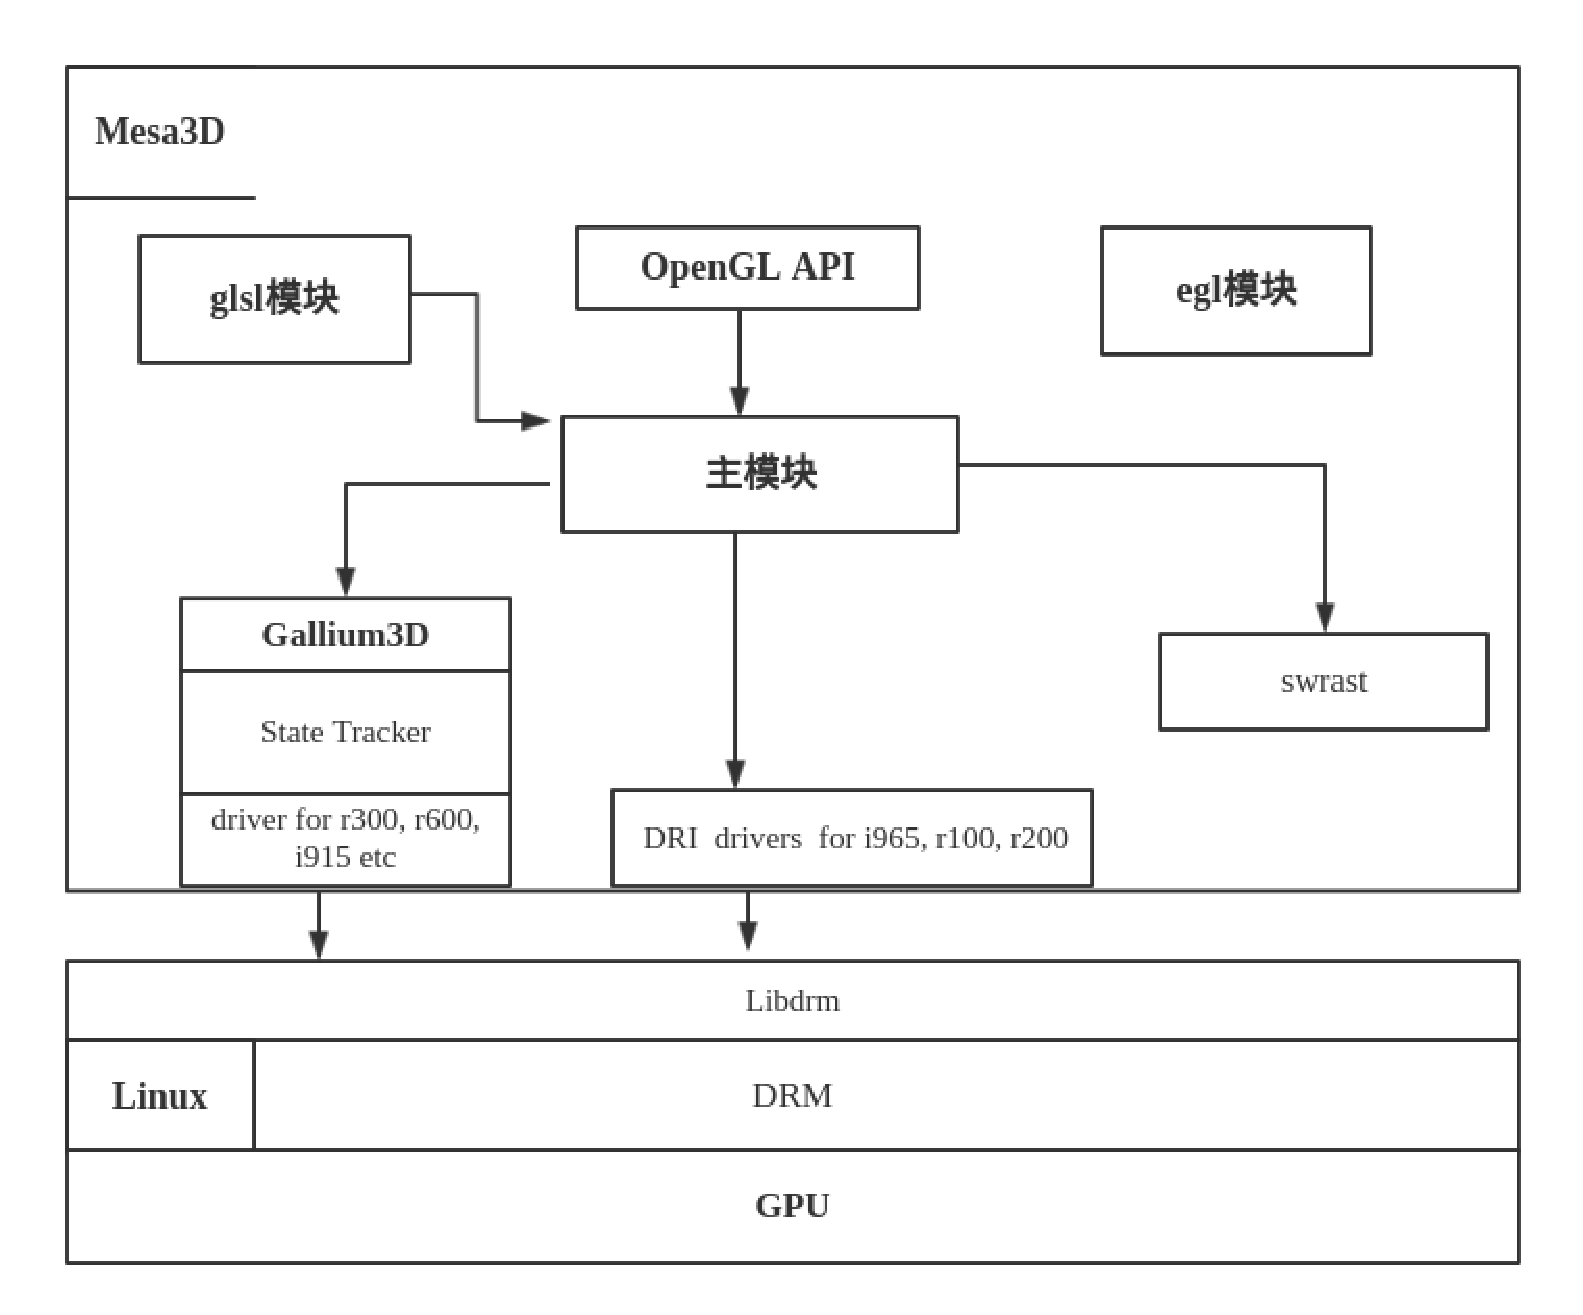
\includegraphics[width=16cm,height=12cm]{figures/chap02/Mesa3D}
  \caption{Mesa3D主要结构}
  \label{fig:Mesa3D}
\end{figure}

下面详细介绍图\ref{fig:Mesa3D}里面的几个模块:

\begin{itemize}
\item{\textbf{主模块}}: \\
Mesa3D的核心模块,它承接所有OpenGL API,并且负责vbo管理、处理glsl编译代码等工作。
\item{\textbf{glsl模块}}: \\
GLSL编译器。此模块将产生Mesa自有的IR(Intermediate Representation)。
\item{\textbf{egl模块}}: \\
EGL库实现模块。此模块是可选模块,在编译Mesa3D时候可配置是否需要。
\item{\textbf{swrast主模块}}: \\
OpenGL API渲染的软件实现模块。例如通过软件实现画点、画线、位图等。
\item{\textbf{DRI Driver for i976 等}}: \\
一些Gallium3D不支持的相关图形硬件的DRI驱动模块,比如i976、r100、r200等GPU。
\item{\textbf{Gallium3D}}: \\
Gallium3D实现模块,用来实现跨图形硬件的渲染技术。
\end{itemize}

其中主模块和Gallium3D模块是论文的研究重点所在。而Gallium3D虽然属于Mesa3D的一个组成部分,但它同样是一个开源的图形项目,它提供一套统一的API,这套API将标准的硬件特性暴露出来,通过Gallium3D将可以与统一的硬件级特性打交道,它是解决图形硬件加速问题的新方法。其主要结构如图\ref{fig:Gallium3D}所示。

\begin{figure}[H] 
  \centering
  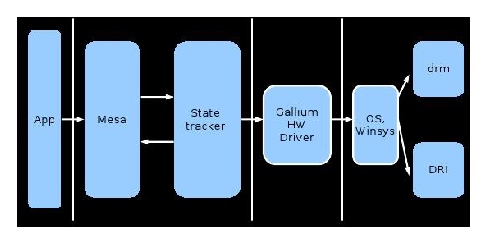
\includegraphics[width=10cm,height=5cm]{figures/chap02/Gallium3D}
  \caption{Mesa3D 模型结构}
  \label{fig:Gallium3D}
\end{figure}

由于Gallium3D不仅支持OpenGL也支持Direct3D等API,所以Gallium3D先是通过其内部的State Tracker模块将Mesa3D主模块的API转化为统一的State Tracker接口,然后接着根据图形硬件信息交给对应图形硬件设备驱动处理,最后调用硬件设备进行硬件加速。


\section{Mesa3D的渲染流程}

%\subsection{Mesa3D的缓存管理}

\section{国内外相关的Mesa3D优化}

\section{本章小结}


\chapter{Mesa3D的性能优化技术}

\section{Mesa3D的CPU与GPU负载平衡的优化}

\subsection{研究背景}

\subsubsection{Radeon R600系列显卡命令处理机制}
Radeon R600显卡提供驱动使用命令流(Command Stream)的形式进行对显卡编程:驱动程序将需要对显卡进行配置的一连串命令写入命令缓冲区,写完之后进入让出处理器,显卡按照命令写入的顺序执行这些命令,执行完成后触发中断通知驱动。具体来说就是CPU将这些命令放入一个称为命令环的环形缓冲区中,命令环是GTT内存中分出来的一片内存,驱动程序往命令环中填充命令,填充完后通知GPU已经写入命令,接着GPU的命令处理器CP(Command Processor)接收并解析驱动程序发送过来的命令流,将解析后的数据传输给图形控制器的其他模块,包括3D图形处理器、2D图形处理器、视频处理器。

\begin{figure}[H] 
  \centering
  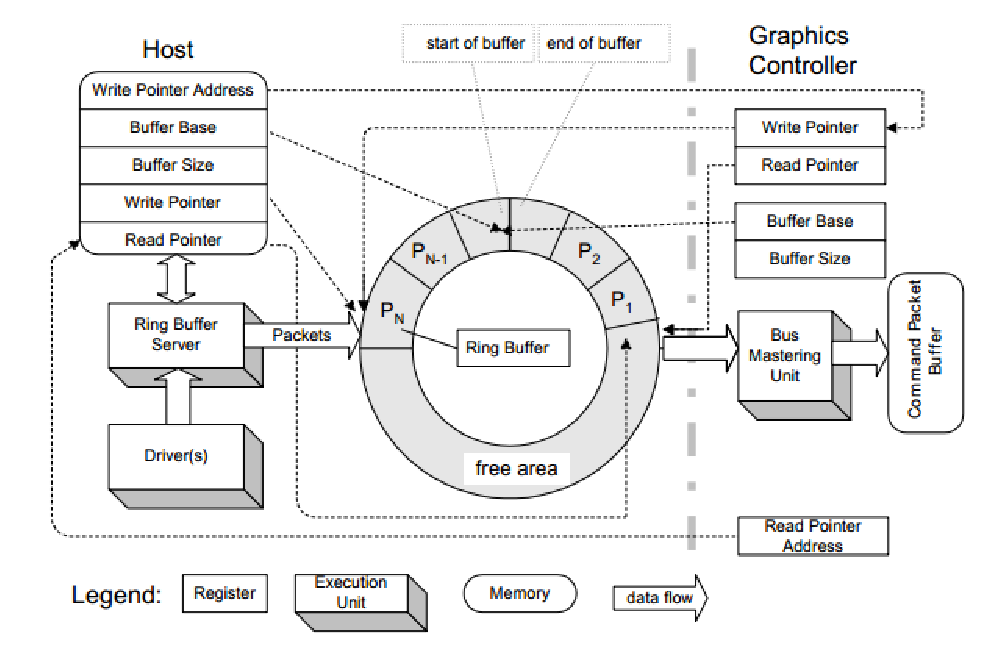
\includegraphics[width=16cm,height=12cm]{figures/chap03/CommandBuffer}
  \caption{Radeon R600系列显卡命令处理机制}
  \label{fig:CommandBuffer}
\end{figure}

如图\ref{fig:CommandBuffer},左边的Host(CPU)和右边的GPU各自记录了命令环的起始地址,并各自保存了一份读写指针,CPU写之前首先查询读指针,确认有空闲空间之后写入内容并更新写指针,GPU读取了命令之后更新读指针。CPU和GPU都要共同维护和管理环形缓冲区的状态:基地址、长度、写指针和读指针。为了使Ring Buffer能够正常工作,CPU和GPU必须维护这种状态的一致性。Ring Buffer基地址和大小是在系统第一次启动时已经初始化好的,之后一般也不会改变。当操作Ring Buffer时, 读指针和写指针的修改非常频繁。为了维护环形缓冲区的状态一致性,当写操作者(CPU)更新写指针时,它必须将写指针告诉GPU。同样的,当读操作者(GPU)更新读指针时,它必须将读指针告知CPU。无论是CPU还是GPU都是从低地址开始进行填写或抽取操作的,一旦到了环形缓冲区的结束处,又从环形缓冲区起始处继续\cite{Radeon-Manual}。  

上面提到的Radeon显卡命令是以命令包的形式出现的,如今Radeon系列显卡有4中命令包,分别是0型、1型、2型和3型命令包,命令包由两部分组成,第一部分是命令包头,第二部分是命令包主体,命令包头为请求GPU执行的具体操作,命令主体为执行该操作需要的数据。

下面分别介绍一下这四种命令包:

\begin{itemize}

\item{\textbf{0型命令包}} \\
0型命令包用于写连续N个寄存器。包主体部分是依次往这些寄存器写的值。包头各个部分的意义为:
\vspace{6pt}
\begin{center} \tablecaption{0型命令包 \label{tab:0-command}} 
\tablefirsthead{
\rowcolor[gray]{0.8}
\multicolumn{1}{l}{\textbf{位}} &
\multicolumn{1}{l}{\textbf{域名称}} &
\multicolumn{1}{c}{\textbf{描述}} \\ }
\tablehead{\multicolumn{3}{c}{
\small 表 \ref{tab:0-command} (续) } \\
\rowcolor[gray]{0.8}
\multicolumn{1}{l}{\textbf{位}} &
\multicolumn{1}{l}{\textbf{域名称}} &
\multicolumn{1}{c}{\textbf{描述}} \\ }
\tabletail{\bottomrule
\multicolumn{3}{c}{\small 接下页} \\}
\tablelasttail{\bottomrule}

\begin{supertabular}{p{2.cm}p{3.cm}m{10.cm}}
	12:0 & BASE\underline{ }INDEX & 要写的连续寄存器的第一个寄存器地址,最大地址0x7FFF \\
	14:13 & 保留位 & \\
	15 & ONE\underline{ }REG\underline{ }WR &  \\ 
	& & \tabitem 0表示将包主体的数据依次写入寄存器中 \\
	& & \tabitem 1表示所有数据写入同一个寄存器 \\
	29:16 & COUNT & 要写的寄存器数目N-1 \\
	31:30 & TYPE & 包类型,0型命令包类型名为0 \\
\end{supertabular}
\end{center}
\vspace{6pt}


\item{\textbf{1型命令包}} \\
1型命令包用于写两个的寄存器,1型命令包包头定义如下:
\vspace{6pt}
\begin{center} \tablecaption{1型命令包 \label{tab:1-command}} 
\tablefirsthead{
\rowcolor[gray]{0.8}
\multicolumn{1}{l}{\textbf{位}} &
\multicolumn{1}{l}{\textbf{域名称}} &
\multicolumn{1}{c}{\textbf{描述}} \\ }
\tablehead{\multicolumn{3}{c}{
\small 表 \ref{tab:1-command} (续) } \\
\rowcolor[gray]{0.8}
\multicolumn{1}{l}{\textbf{位}} &
\multicolumn{1}{l}{\textbf{域名称}} &
\multicolumn{1}{c}{\textbf{描述}} \\ }
\tabletail{\bottomrule
\multicolumn{3}{c}{\small 接下页} \\}
\tablelasttail{\bottomrule}

\begin{supertabular}{p{2.cm}p{3.cm}m{10.cm}}
	10:0 & REG\underline{ }INDEX1 & 第一个寄存器的地址 \\
	22:11 & REG\underline{ }INDEX2 & 第二个寄存器的地址 \\
	29:22 & RESERVED & 保留位 \\
	31:30 & TYPE & 1型命令包的类型为0x1 \\
\end{supertabular}
\end{center}
\vspace{6pt}

\item{\textbf{2型命令包}} \\
2型命令包是一个空命令包,用于填充对齐命令。2型命令包没有包主体,其包头最高两位为0x2,其它位无意义。

\item{\textbf{3型命令包}} \\
3型命令包是最功能最丰富的包,图形的主要功能都是通过这类包实现的。3型命令包主体内容由包头的IT\underline{ }OPCODE决定。3型命令是主要的命令包,涵盖了寄存器设置/绘图命令/同步等主要操作。3型命令包包头定义如下:
\vspace{6pt}
\begin{center} \tablecaption{3型命令包 \label{tab:3-command}} 
\tablefirsthead{
\rowcolor[gray]{0.8}
\multicolumn{1}{l}{\textbf{位}} &
\multicolumn{1}{l}{\textbf{域名称}} &
\multicolumn{1}{c}{\textbf{描述}} \\ }
\tablehead{\multicolumn{3}{c}{
\small 表 \ref{tab:3-command} (续) } \\
\rowcolor[gray]{0.8}
\multicolumn{1}{l}{\textbf{位}} &
\multicolumn{1}{l}{\textbf{域名称}} &
\multicolumn{1}{c}{\textbf{描述}} \\ }
\tabletail{\bottomrule
\multicolumn{3}{c}{\small 接下页} \\}
\tablelasttail{\bottomrule}

\begin{supertabular}{p{2.cm}p{3.cm}m{10.cm}}
	7:0 & reserved & 保留位 \\
	15:8 & IT\underline{ }OPCODE & 操作码 \\
	29:16 & COUNT & 包主题DWORDS数目-1 \\
	31:30 & TYPE & 3型包类型为0x3 \\
\end{supertabular}
\end{center}
\vspace{6pt}
\end{itemize}

\subsubsection{Mesa3D显示列表绘制模式实现原理}
\label{sec:display-list}

显示列表绘制模式即glGenList/glNewList/glEndList/glCallList,它可以提高性能,因为它存储OPENGL的函数,供以后使用,如果需要多次重绘同一个几何图形,或者如果一次需要多次调用的用于更改状态的函数,把这些函数存储在显示列表中,此时将显示列表中的矩阵结果集保存,后续使用不需要重复计算以提高性能。显示列表更像是命令缓存器,而不是动态数据库,也就是说当显示列表创建后,就无法修改。同时显示列表的创建也存在一定的系统开销,因此一个小的显示列表未必会提升性能。

我们以下面所示的svPerfGL测试集里面的显示列表模式为例,来看一下Mesa3D图形库是如何实现显示列表的绘制模式的。

\begin{lstlisting}
 // Create Display List
 glNewList(trianglesListIndx, GL_COMPILE);
 glDrawArrays(GL_TRIANGLES, 0, tNumVerts);
 glEndList(); 

 // Call Display List
 glCallList(trianglesListIndx);
\end{lstlisting}


当执行glNewList时,Mesa3D图形库会执行alloc\underline{ }vertex\underline{ }store函数预分配大小为VBO\underline{ }SAVE\underline{ }BUFFER\underline{ }SIZE*sizeof(GLfloat)的空白VRAM空间,这个空间我们姑且称之为buffer0。在显示列表机制下,保存模式的glDrawArrays只会执行一次,目的是将所有的顶点属性(位置、法线和颜色等)写入buffer0。VBO\underline{ }SAVE\underline{ }BUFFER\underline{ }SIZE的初值是8*1024,只能存放8*1024/3=2730个顶点属性,而glDrawArrays可能需要写入更多的顶点属性,因此buffer0是远远不够存放这些顶点属性的。当buffer0溢出后,显示列表会继续分配大小为VBO\underline{ }SAVE\underline{ }BUFFER\underline{ }SIZE * sizeof(GLfloat)的buffer1,buffer2,buffer3...直到所有顶点属性都写入VRAM。可见,当glDrawArray执行完时,所有的顶点属性已经存入VRAM,但是分散在很多个小buffer中。

接着通过执行glCallList来调用已保存好顶点属性的显示列表,glCallList将执行vbo\underline{ }save\underline{ }playback\underline{ }vertex\underline{ }list函数来实现渲染,该函数调用r600\underline{ }draw\underline{ }vbo向GPU发如下命令:

\begin{lstlisting}
cs->buf[cs->cdw++] = PKT3(PKT3_DRAW_INDEX_AUTO, 1, 
                          rctx->predicate_drawing);
cs->buf[cs->cdw++] = info.count;
cs->buf[cs->cdw++] = V_0287F0_DI_SRC_SEL_AUTO_INDEX 
                     | (info.count_from_stream_output? 
                        S_0287F0_USE_OPAQUE(1) : 0);
\end{lstlisting}

这些命令通过Command Stream机制被GPU读取并执行,从而启动pipeline进行3D渲染。

\begin{figure}[H] 
  \centering
  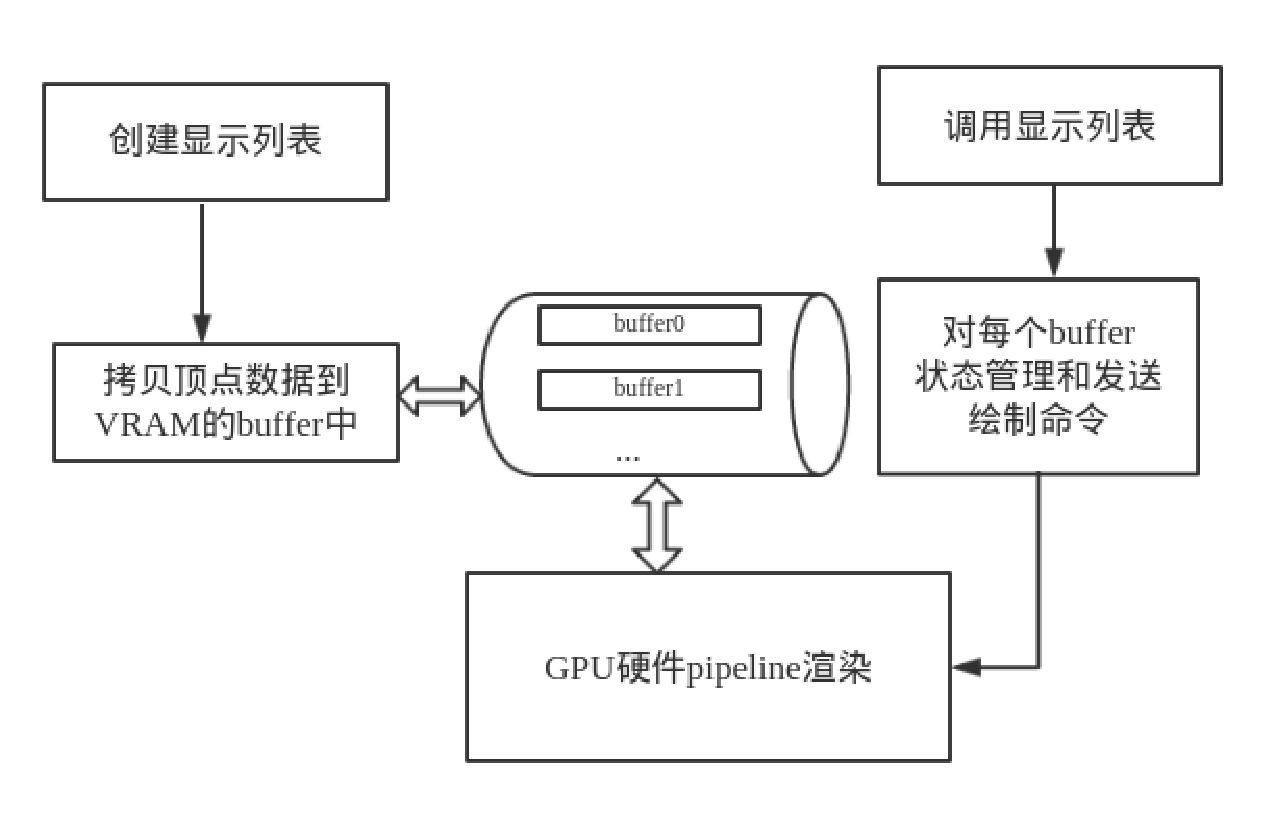
\includegraphics[width=12cm,height=10cm]{figures/chap03/display-list-flow}
  \caption{Mesa3D图形库显示列表实现机制}
  \label{fig:display-list-flow}
\end{figure}

由于显示列表是一次创建多次调用,所以如图\ref{fig:display-list-flow}所示,每次在调用显示列表时候都会做对每个buffer进行状态管理和发送绘制命令到GPU。GPU在执行完3D渲染之后将结果放入framebuffer中然后通过显示设备显示出来。

\subsection{CPU与GPU负载分析}

我们在前面就介绍过Radeon R600系列GPU的工作模型就是CPU端将数据和命令写入Command Buffer中,然后GPU读取Command Buffer中的命令并执行(图\ref{fig:CommandBuffer})。所以从这个模型我们可以看到这里存在着CPU/GPU的负载平衡问题:如果CPU端执行效率比GPU端执行效率更快,那么会导致Command Buffer满载,这样CPU就不得不需要同步操作停下来等待GPU处理完命令以得到Command Buffer里面一些空闲的位置继续写入命令;同样,如果GPU端执行的效率更高,这样每当CPU写完命令之后GPU就可以很快的执行完毕,这样Command Buffer常常会处于空闲状态,GPU就不得不空闲下来等待CPU的处理结果。不论是哪一种情况都属于CPU与GPU的负载不平衡,这样都会造成性能的瓶颈。

从前面的分析里面我们可以知道显示列表模式的CPU和GPU的协同工作模型就是:CPU数据准备与状态管理、GPU处理数据、CPU数据准备与状态管理、GPU处理数据、反复直至数据全部处理完毕。那么现在我们就从CPU与GPU的负载平衡的关系上来看我们将上面提到的svPerfGL里面的显示列表模式测试项的情况。这里测试每帧100万个三角形的绘制时候CPU和GPU的负载状况。测试结果如下图\ref{fig:cpu-load-dsp}和图\ref{fig:gpu-load-dsp}

\begin{figure}[H]
  \begin{minipage}[t]{0.5\linewidth} 
  \centering
  \includegraphics[width=8cm,height=6cm]{figures/gnuplot/dsp/cpu-load}
  \caption{显示列表测试项CPU负载}
  \label{fig:cpu-load-dsp}
  \end{minipage}
  \begin{minipage}[t]{0.5\linewidth} 
  \centering
  \includegraphics[width=8cm,height=6cm]{figures/gnuplot/dsp/gpu-load}
  \caption{显示列表测试项GPU负载}
  \label{fig:gpu-load-dsp}
  \end{minipage}
\end{figure}

从上面的图中我们可以看到CPU的负载情况明显比GPU要大很多,这里的原因也很好解释: 如前面章节\ref{sec:display-list}研究的那样,对每一次的buffer,Mesa3D需要都先在CPU端数据准备和状态管理,然后提交给GPU处理。这里当我们绘制大量的顶点时候,例如glDrawArray函数里面写入100万个三角形,那么每个三角形需要有3个顶点*3钟顶点属性(位置、法线和颜色),所以一种有1000000*3*3即9000000个顶点属性,根据前面分析的默认的buffer大小是8*1024*4字节,那么总共需要的buffer数目就是9000000*3*4/(8*1024*4)即3296个。由于对这3296个buffer每一个都需要CPU进行进行数据准备和状态管理等大量操作,这对性能较为优越的X86不是问题,却能极大的消耗龙芯3A的CPU。这样也就造成了CPU负载过大,而GPU负载较小的结果。


\subsection{CPU与GPU负载平衡优化}

由前一节分析我们可以看到CPU负载过大导致了CPU与GPU负载不平衡问题,究其原因就是CPU端需要处理的buffer数目过多,于是本文提出了一种通过调整显示列表缓存buffer大小的方法来优化显示列表的CPU与GPU负载不平衡问题。

如前面章节\ref{sec:display-list}所分析的那样,显示列表由于数据都已经上传保存到VRAM中的buffer里面,所以每次调用显示列表时候并不需要再次上传数据,而只是对每个buffer进行数据准备和状态管理即可,这些工作与buffer所装载的数据大小并没有关系,于是我们可以将buffer的大小调整到一个合适的数值,然后使得CPU的负载降低,GPU的负载增加以提高整体性能。

为了寻找显示列表缓存buffer的合适大小,我们通过测试svPerfGL显示列表程序在60秒内绘制每帧100万个三角形的绘制性能来确定这一合适值。相关测试结果如下表\ref{tab:buffer-performance}:

\begin{center} \tablecaption{svPerfGL显示列表测试项不同buffer大小下绘制性能 \label{tab:buffer-performance}} 
\tablefirsthead{
\rowcolor[gray]{0.8}
\multicolumn{1}{c}{\textbf{buffer大小}} &
\multicolumn{1}{c}{\textbf{帧数}} &
\multicolumn{1}{c}{\textbf{渲染效率(frame/s)}} \\ }
\tablehead{\multicolumn{3}{c}{
\small 表 \ref{tab:0-command} (续) } \\
\rowcolor[gray]{0.8}
\multicolumn{1}{c}{\textbf{buffer大小}} &
\multicolumn{1}{c}{\textbf{帧数}} &
\multicolumn{1}{c}{\textbf{渲染效率(frame/s)}} \\ }
\tabletail{\bottomrule
\multicolumn{3}{c}{\small 接下页} \\}
\tablelasttail{\bottomrule}

%./svPerfGL -i ../../trisNormsColors-512.nc -w 1280 -h 1024 -2 -r -t 60 -s 3000000
\begin{supertabular}{p{6.cm}p{3.cm}m{6.cm}}
	32K& 169& 2.81\\
	64K& 250& 4.16\\
	128K& 241& 4.01\\
	256K& 242& 4.03\\
	512K& 266& 4.42\\
	1024K& 268& 4.46\\
	2048K& 269& 4.47\\
	4096K& 209& 3.47\\
\end{supertabular}
\end{center}

根据测试结果,我们可以发现将buffer的大小设定为2048KB能够取得较好的性能。此时再次测量CPU和GPU的负载状况如图\ref{fig:cpu-load-dsp-opt}和图\ref{fig:gpu-load-dsp-opt}:

\begin{figure}[H] 
  \begin{minipage}[t]{0.5\linewidth} 
  \centering
  \includegraphics[width=8cm,height=6cm]{figures/gnuplot/dsp/cpu-load-opt}
  \caption{显示列表测试项优化后CPU负载}
  \label{fig:cpu-load-dsp-opt}
  \end{minipage}
  \begin{minipage}[t]{0.5\linewidth} 
  \centering
  \includegraphics[width=8cm,height=6cm]{figures/gnuplot/dsp/gpu-load-opt}
  \caption{显示列表测试项优化后GPU负载}
  \label{fig:gpu-load-dsp-opt}
  \end{minipage}
\end{figure}

可以看到此时GPU刚好达到了满载,CPU负载较轻,因为龙芯平台CPU处理能力较GPU的处理能力稍弱,所以这样的负载关系比较符合当前硬件特点,所以能够取得较好的性能提升。

当然buffer大小调整这种优化方法也有一定的缺点,我们将buffer的大小调大的时候会增加VRAM的管理粒度,在小数据规模时候可能会造成VRAM的浪费,特别是在某些显卡显存比较紧俏的机器环境下可能会消耗掉所有的VRAM空间,造成VRAM空间不够程序无法执行的问题。所以这个优化方法可以作为可配置的优化手段,在实际工程应用中可以根据具体硬件情况进行选择。


\newpage
\section{Mesa3D的内存到显存的数据传输的优化}

\subsection{研究背景}

\subsubsection{Mesa3D顶点数组绘制模式实现原理}
从前面的立即模式实现原理我们可以看到顶点数据是一个个的搬运到VRAM上的buffer上的,当我们绘制拥有大量数据的图形时候,这样一点点的搬运就显得非常的缓慢了,当然我们可以尝试使用显示列表来对这些数据进行预编译,需要遍历这些顶点数据然后把数据传给GPU的显存。但是这些数据不一定是静态的,有可能在我们每次渲染的时候,我们需要对这些数据进行更改。这个时候就不适合使用显示列表了。

为了很好的解决这个问题。我们可以使用顶点数组,我们可以随时进行预编译或修改几何图形,然后一次性传输这些数据。顶点数组的绘制模式相对于立即模式极大的提高了绘制效率。使用顶点数组有3个基本的步骤:

\begin{itemize}
\item{} 激活(启用)最多可达8个数组,每个数组用于存储不同类型的数据: 顶点坐标,表面法线,颜色等等。
\item{} 把数据放入数组中。这些数组是通过它们的内存位置的地址(即指针)进行访问。
\item{} 用这些数据绘制几何图形。OpenGL通过指针从所有激活的数组中获取数据。
\end{itemize}

我们还是以svPerfGL的顶点数组模式测试项为研究对象来分析Mesa3D顶点数组的实现原理:

\begin{lstlisting}
glEnableClientState(GL_VERTEX_ARRAY);
glVertexPointer(3, GL_FLOAT, sizeof(float)*3, (const GLvoid *)tVerts);
glEnableClientState(GL_NORMAL_ARRAY);
glNormalPointer(GL_FLOAT, sizeof(float)*3, (const GLvoid *)tNorms);
glEnableClientState(GL_COLOR_ARRAY);
glColorPointer(3, GL_FLOAT, sizeof(float)*3, (const GLvoid *)tColors);

glDrawArrays(GL_TRIANGLES, 0, tNumVerts);
\end{lstlisting}

这里在介绍Mesa3D顶点数组实现原理之前先介绍一个重要的数据结构:
\begin{lstlisting}
struct pipe_vertex_buffer{
   ...
   struct pipe_resource *buffer; 
   const void *user_buffer;
};

struct pipe_vertex_buffer vertex_buffer[PIPE_MAX_ATTRIBS];
\end{lstlisting}
这里vertex\underline{ }buffer数组就是存放着各个属性数据数组的指针,当我们使用传统的立即模式时候,这些指针就指向着前面一节说到的VRAM上的buffer(struct pipe\underline{ }resource *buffer),而在我们使用顶点数组模式时候,这些指针就指向着我们用户准备的顶点数据数组(const void *user\underline{ }buffer)。所以在顶点数组模式下,在glVertexPointer()这类函数执行时候,Mesa3D会把用户指定的数组指针添加到对应vertex\underline{ }buffer[]数组里面的user\underline{ }buffer中。接着我们调用glDrawArrays()之类的函数进行顶点数组模式绘制时候,Mesa3D会执行u\underline{ }vbuf\underline{ }upload\underline{ }buffers函数将用户定义的顶点数组数据通过memcpy()函数从内存拷贝到显存中,然后像之前的立即模式一样向GPU发送绘制命令执行硬件渲染。

\begin{figure}[H] 
  \centering
  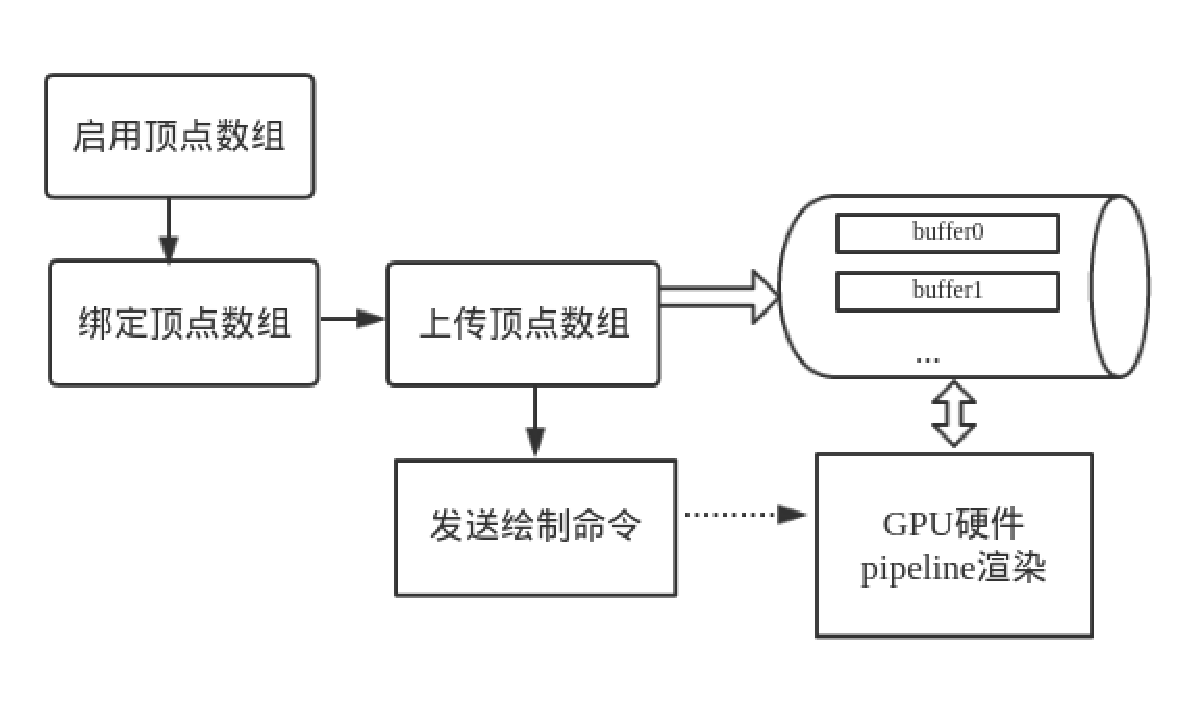
\includegraphics[width=12cm,height=8cm]{figures/chap03/vbo-flow}
  \caption{Mesa3D图形库顶点数组模式实现机制}
  \label{fig:vbo-flow}
\end{figure}

顶点数组模式绘制的简要流程如图\ref{fig:vbo-flow}所示,这里需要说明的是顶点数组模式下在VRAM上创建的buffer大小是依据用户定义的数组大小而定的,并不像立即模式那样有着固定的大小,一旦填满就开始部分绘制,顶点数组模式是把所有数据都传递到显存之后再一次性的GPU绘制,由于是一次性memecpy的大数据传输,所以传输效率上要比传统的立即模式快的多,这也是后来OpenGL标准中增加顶点数组模式的原因。

\subsubsection{内存与显存数据传输优化的意义}

在一般的GPU硬件加速的程序应用场景中,内存到显存的数据传输是不可避免的,Chris Gregg等人在论文Where is the Data? Why You Cannot Debate CPU vs. GPU Performance Without the Answer\cite{Where-is-the-Data}里面以十多项常见的GPU应用程序为benchmark,通过测试和分析不同数据规模下的benchmark运行效率发现内存与显存之间的数据传输几乎对所有的GPU应用程序运行性能都有着十分重要的影响。特别是在大数据输入集下,内存与显存传输的时间开销最高可以达到GPU计算时间开销的50多倍。由此我们可以得到结论:内存与显存的数据传输是影响GPU应用程序性能的重要的因素。


\subsubsection{CPU与GPU的访存机制}

我们首先介绍以下GPU的访存机制。GPU使用的内存分为两个部分,一部分是显卡自带的显存称为VRAM(Vedio RAM),另一部分是系统主存(即CPU端内存)也称为GTT内存。为了实现GPU同时使用VRAM内存和GTT内存最简单的方法就是将这两片内存统一编址,VRAM是显卡自带的内存,它的地址一定是连续的,但是不连续的GTT内存如果要统一编址,那么一定需要通过建立页表映射关系,这个页表也就是GTT(graphics translation table, 地址转换表)。

和CPU的地址类似,GPU直接使用的地址被称为“GPU虚拟地址”,经过查页表转化之后的地址称为“GPU物理地址”,也就是GPU最终真实访问的地址,其中GPU的虚拟地址和物理地址转换过程如图\ref{fig:gpu-mmu}所示:对于属于GTT的虚拟地址,通过查找GPU页表找到真实的PCI地址,然后通过PCI地址访问系统主存;对于属于VRAM的虚拟地址则无须页表转换直接在VRAM内寻址。

\begin{figure}[H] 
  \centering
  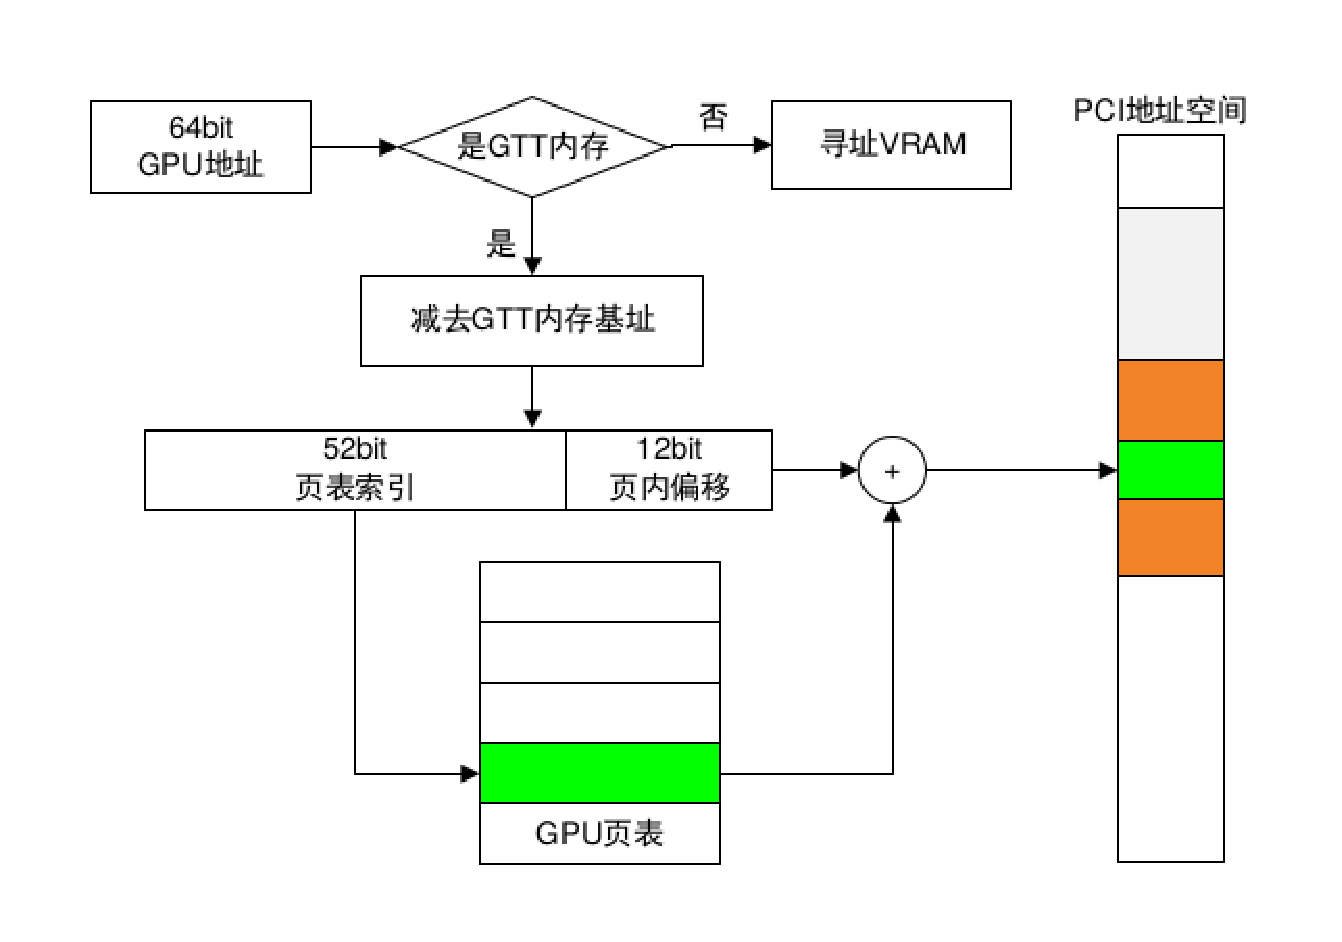
\includegraphics[width=12cm,height=8cm]{figures/chap03/gpu-mmu}
  \caption{GPU的内存访问机制}
  \label{fig:gpu-mmu}
\end{figure}

与此同时,CPU使用的内存就复杂的多了,CPU通过MMU单元将虚拟地址转化成实际的物理地址,这些物理地址有的是系统主存的地址,有些是外接设备的地址,其中就包括GPU的自带显存VRAM地址。通过下图\ref{fig:cpu-gpu-mm}可以看到,CPU和GPU均能自有访问系统内存和显卡内存VRAM。

\begin{figure}[H] 
  \centering
  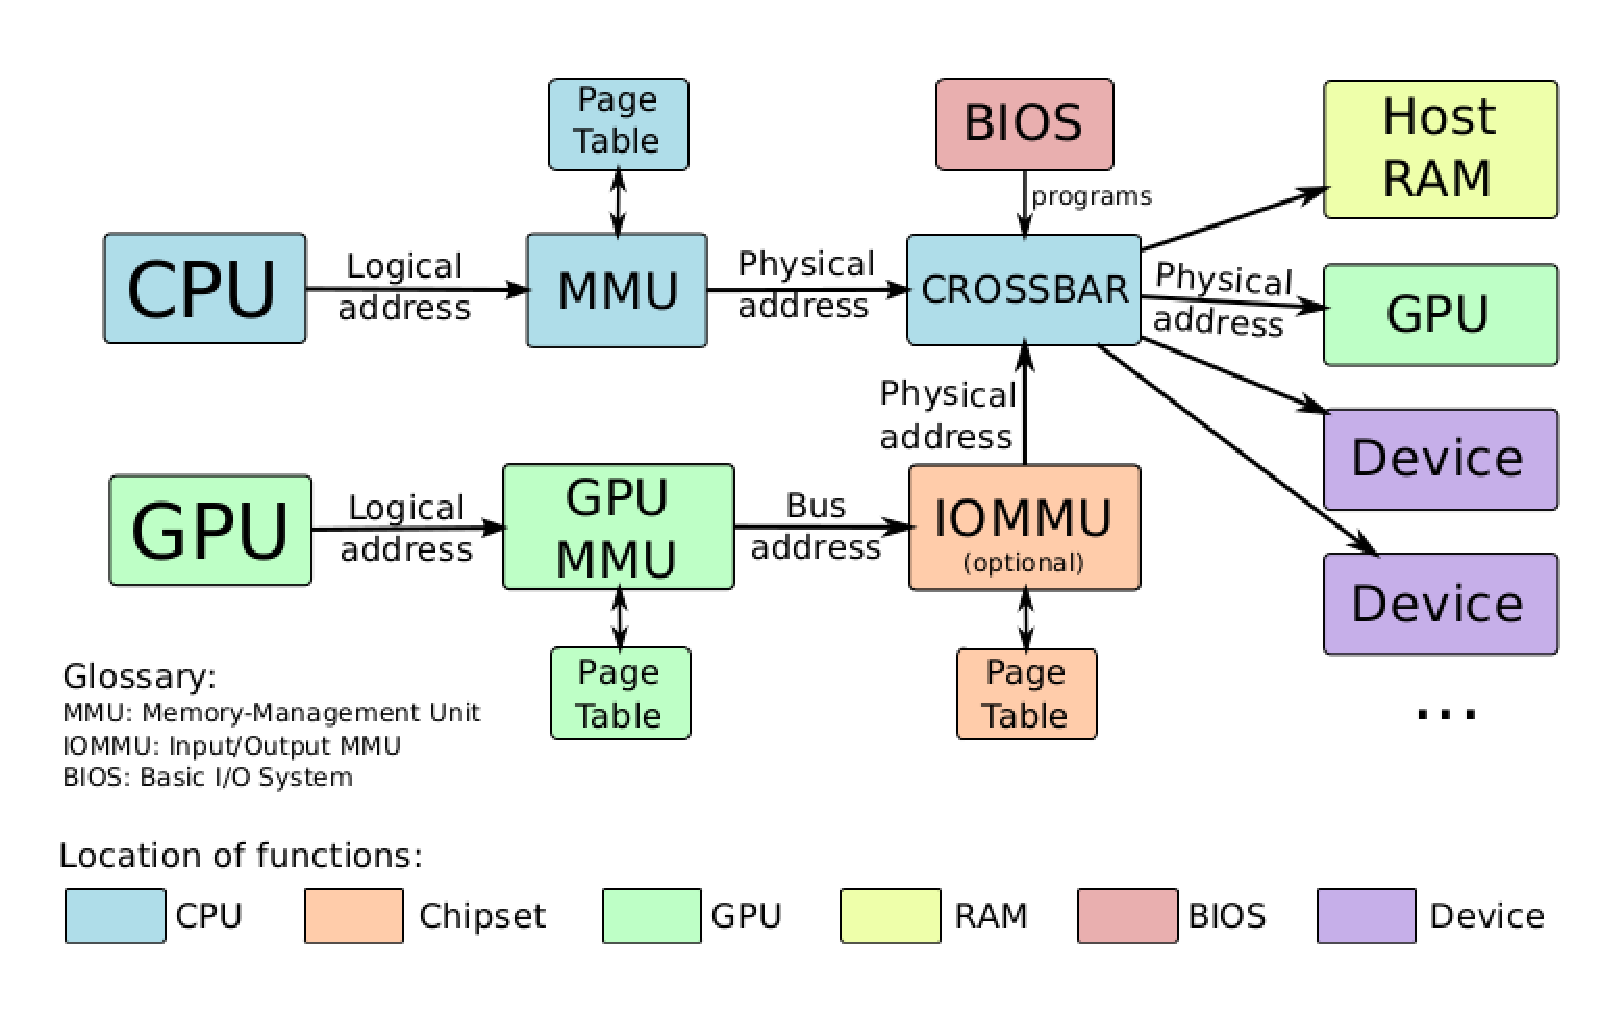
\includegraphics[width=12cm,height=8cm]{figures/chap03/cpu-gpu-mm}
  \caption{CPU与GPU内存请求回路}
  \label{fig:cpu-gpu-mm}
\end{figure}

\subsubsection{龙芯平台下内存与显存传输的性能分析}

从CPU的角度来说我们可以看到存在着两种内存传输: 系统内存到系统内存(cache)、系统内存到显存。这里本文以龙芯3A搭载Radeon R600显卡平台为例测试并研究这两种传输的性能。得到相关数据如下表\ref{tab:memcpy-performance}所示:

\begin{center} \tablecaption{龙芯3A访存性能分析 \label{tab:memcpy-performance}} 
\tablefirsthead{
\rowcolor[gray]{0.8}
\multicolumn{1}{c}{\textbf{数据量大小}} &
\multicolumn{1}{c}{\textbf{内存到内存}} &
\multicolumn{1}{c}{\textbf{内存到显存}} \\ }
\tablehead{\multicolumn{3}{c}{
\small 表 \ref{tab:memcpy-performance} (续) } \\
\rowcolor[gray]{0.8}
\multicolumn{1}{c}{\textbf{数据量大小}} &
\multicolumn{1}{c}{\textbf{内存到内存}} &
\multicolumn{1}{c}{\textbf{内存到显存}} \\ }
\tabletail{\bottomrule
\multicolumn{3}{c}{\small 接下页} \\}
\tablelasttail{\bottomrule}

%./svPerfGL -i ../../trisNormsColors-512.nc -w 1280 -h 1024 -2 -r -t 60 -s 3000000
\begin{supertabular}{p{5.cm}<{\centering}p{5.cm}<{\centering}m{6.cm}<{\centering}}
	4KB& 409MB/s& 12MB/s\\
	16KB& 564MB/s& 14MB/s\\
	64KB& 313MB/s& 14MB/s\\
	256KB& 268MB/s& 14MB/s\\
	1MB& 246MB/s& 14MB/s\\
	4MB& 210MB/s& 14MB/s\\
	16MB& 201MB/s& 14MB/s\\
	64MB& 185MB/s& 14MB/s\\
	256MB& 178MB/s& 14MB/s\\
\end{supertabular}
\end{center}

通过上表\ref{tab:memcpy-performance}我们可以发现龙芯3A平台上内存到显存拷贝效率较低,这里主要是因为内存到显存拷贝数据传输是通过PCI-E总线传输的,而龙芯平台上PCI-E带宽非常的小,所以导致这样直接传输的性能底下。

\subsection{Mesa3D图形库CPU与GPU访存行为分析}

在Mesa3D图形库的实现中,CPU端在初始化过程中会创建顶点对象缓存区,而这些顶点对象缓存区是创建在VRAM之上的,然后通过内存映射的方式映射成CPU端虚拟地址进行访问。在上层程序需要使用Mesa3D进行图形绘制时候,Mesa3D会将绘制相关的顶点数据拷贝到顶点对象缓存区中,即发生了CPU端内存到显存的拷贝,整个过程是同步实现的,即需要占用CPU的指令周期。当GPU接受到绘制命令和相关顶点数据准备好时候,GPU就开始内部的硬件图形加速渲染管线进行图形渲染,并将渲染结果放置到显存的framebuffer中以待显示。以svPerfGL程序顶点数组测试项为例,假如我们需要每帧绘制100万个三角形,那么就会发生三次顶点数据拷贝,分别是顶点位置、顶点颜色和顶点法向量信息,每次拷贝数据量是100万*3*3*4B即36MB数据的大小。

通过上表\ref{tab:memcpy-performance}我们可以看到从内存拷贝到显存这么多数据是非常缓慢的,并且我们通过perf工具测试出整个顶点数组模式测试项的执行时间中百分之九十的时间都花在这个拷贝数据之上,所以成为了程序的性能瓶颈。

\subsection{Mesa3D图形库CPU与GPU访存优化}

针对Mesa3D图形库实际的访存特点,本文从访存策略与拷贝效率这两个方面提出了相应的优化方案。

\subsubsection{CPU与GPU访存策略的优化}
从前面的介绍我们知道,由于CPU端内存到显存的数据拷贝效率低下,导致占用了大量的CPU执行周期,使得CPU执行时间占比过大,而GPU相对执行时间过少。为了改变这一状况,如下图\ref{fig:vbo-gtt}我们可以把顶点数据缓冲区创建在系统内存之上,CPU只需简单的系统内存内部搬运数据,而GPU则通过GTT的方式访问顶点数据缓冲区然后进行图形硬件渲染。

\begin{figure}[H] 
  \centering
  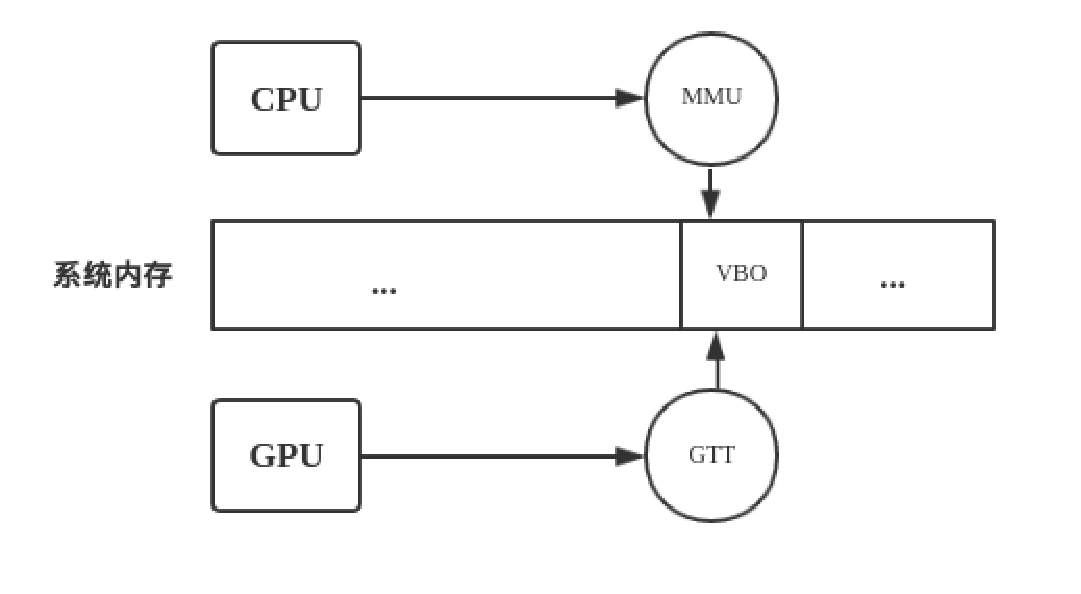
\includegraphics[width=10cm,height=6cm]{figures/chap03/vbo-gtt}
  \caption{Mesa3D图形库CPU与GPU改进后访存策略}
  \label{fig:vbo-gtt}
\end{figure}

虽然这样之后,GPU渲染时候的数据访问效率会降低,但是由于本身GPU工作负担小于CPU,而且因为龙芯平台CPU执行效率相对GPU较弱,所以整个CPU和GPU的并行程度提高了,缩短了整个的执行时间。

\subsubsection{CPU拷贝效率的优化}

在前一节的改进访存策略之后,我们可以通过提高拷贝效率来改进CPU的数据传输性能。由于CPU端向GTT的数据拷贝大多都是单精度浮点数据的拷贝,所以我们可以通过龙芯平台特有的宽位访存指令来提高拷贝效率。

\textbf{龙芯扩展宽位访存指令}: 龙芯平台为了自身发展的需求,通过龙芯指令系统融合技术\cite{loongson-merge},专门开发了一些宽位访存指令,诸如本文使用到的128bit浮点访存指令GSLQ和GSSQ可以实现128bit的浮点数据存取。

由于我们的宽位访存指令GSLQ和GSSQ必须要按照要求先进行128位对齐后使用,所以我们在优化CPU的单精度浮点数据拷贝时候,则必须要考虑到拷贝源地址和目的地址的对齐情况,为了更简明的说明这个问题,我们可以通过下图\ref{fig:memcpy}来看宽位访存指令实现拷贝效率优化的整个过程。

\begin{figure}[H] 
  \centering
  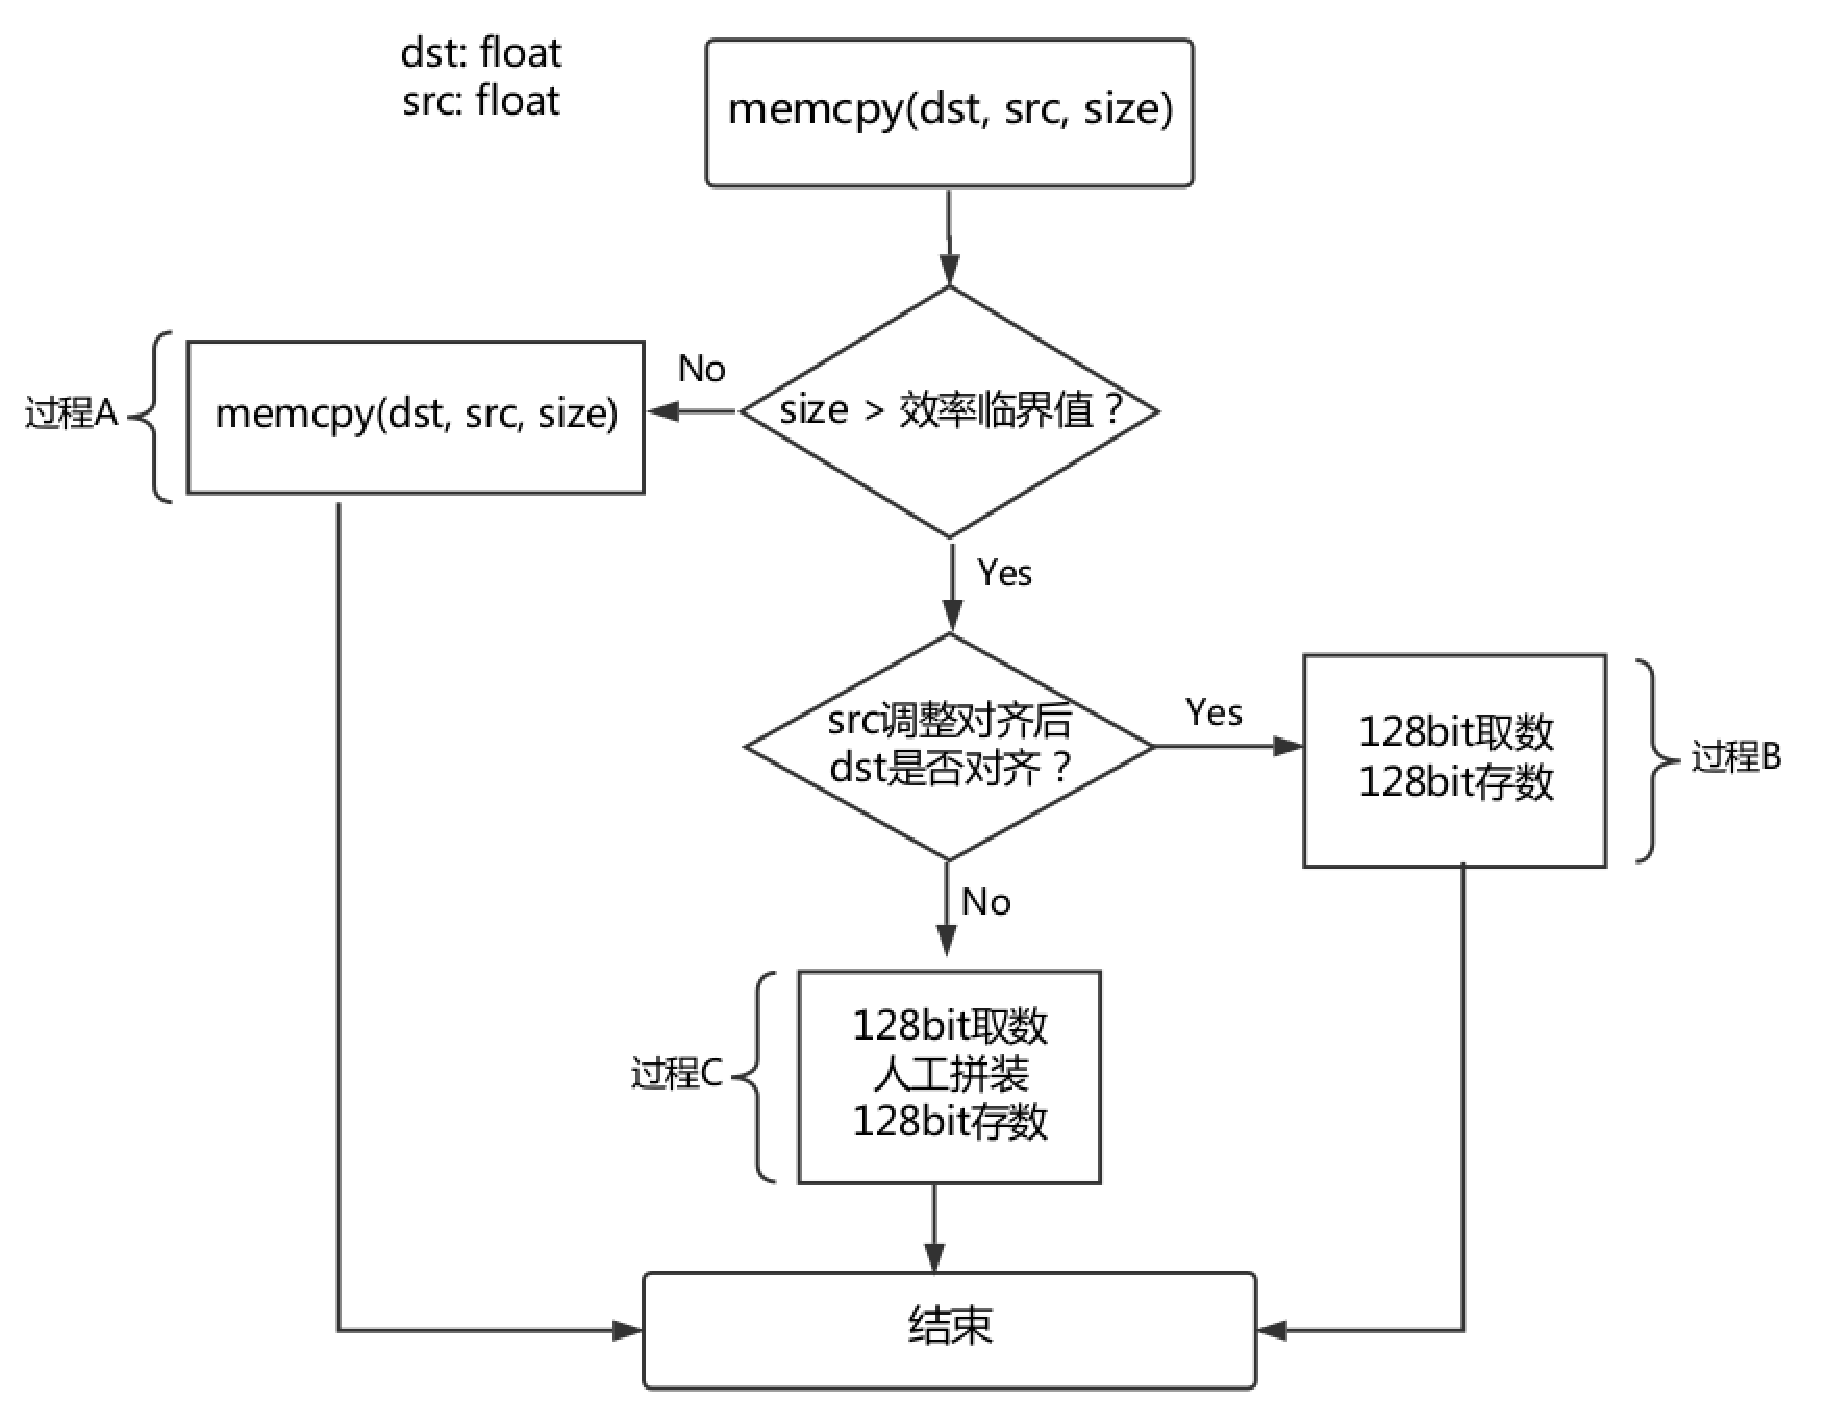
\includegraphics[width=16cm,height=9cm]{figures/chap03/memcpy}
  \caption{宽位访存指令实现拷贝效率优化}
  \label{fig:memcpy}
\end{figure}

这里介绍一下流程图\ref{fig:memcpy}里面的过程A、过程B和过程C的具体工作:

\begin{itemize}

\item{\textbf{过程A}}: 直接调用glibc系统库的memcpy函数。
\item{\textbf{过程B}}: \\
因为这种情况下源地址src和目的地址dst都是128bit对齐的,所以只需要直接的使用宽位访存指令取数和存数即可。相关实现伪代码如下:
\vspace{6pt}
\begin{breakablealgorithm}
	\caption{过程B算法}
	\begin{algorithmic}[1] %每行显示行号
		\Require $dst$目的地址,$src$源地址, $size$大小
		%\Ensure 
		\Function {memcpy}{$dst, src, size$}
			\State $gpr0 \gets src$
			\State $gpr1 \gets dst$
			\State $off \gets 0$
			\While {$off + 16 < size$}
				\State $gslq\, gpr2,\, gpr1,\, off(gpr0)$
				\State $gssq\, gpr2,\, gpr1,\, off(gpr1)$
				\State $off \gets off + 16$
			\EndWhile
		\EndFunction
	\end{algorithmic}
\end{breakablealgorithm}
\vspace{6pt}

\item{\textbf{过程C}}: \\
由于在源地址src对齐后,目的地址dst不是128bit对齐的,所以这里目的地址dst与128bit对齐地址的差可能会是32bit、64bit和96bit这三种,然后无论哪一种都需要我们进行人工的暂存和拼接组装。实现伪代码如下:
\vspace{6pt}
\begin{breakablealgorithm}
	\caption{过程C算法}
	\begin{algorithmic}[1] %每行显示行号
		\Require $dst$目的地址,$src$源地址, $size$大小
		%\Ensure 
		\Function {memcpy}{$dst, src, size$}
			\State $array pre[0:3] \gets \{0.0f, 0.0f, 0.0f, 0.0f\}$
			\State $array cur[0:3] \gets \{0.0f, 0.0f, 0.0f, 0.0f\}$
			\State $offbit \gets (dst \% 16) * 8$
			\State $n \gets offbit/32 - 1$
			\State $pre[0:n] \gets src[0:n]$
			\State $off \gets 16$
			\State $gpr0 \gets src + off$
			\State $gpr1 \gets dst + off - offbit/8$
			\While {$off + 16 < size$}
				\State $gslq\, gpr2, gpr3, off(gpr0)$
				\State $cur[n+1:3]  \gets \{gpr2, gpr3\}\, low\, 128-offbit\, bit$
				\State $cur[0:n] \gets pre[0:n]$
				\State $pre[0:n] \gets \{gpr2, gpr3\}\, high\, offbit\, bit$
				\State ${gpr2, gpr3} \gets cur[0:3]$
				\State $gssq\, gpr2,\, gpr3,\, off(gpr1)$
				\State $off \gets off + 16$
			\EndWhile
		\EndFunction
	\end{algorithmic}
\end{breakablealgorithm}
\vspace{6pt}

\end{itemize}

这里以目的地址dst与128bit对齐地址偏移32bit为例来解释上述过程C算法。如下图\ref{fig:offset32}所示,我们需要将src开始的源数据搬运到dst开始的目的位置,此时src已经是128bit对齐,而dst与128bit对齐相差32bit,这时我们将s4位置的32bit数据暂存起来,接着采用宽位访存指令读取src下一个128bit数据,即\{s5,s6,s7,s8\},接着我们将s4,s5,s6,s7拼装起来成128bit采用宽位访存指令存储到dst的下一个128bit对齐位置,即{d4,d5,d6,d7}。以此规律循环处理即可完成非对齐情况下的数据拷贝。


\begin{figure}[H] 
  \centering
  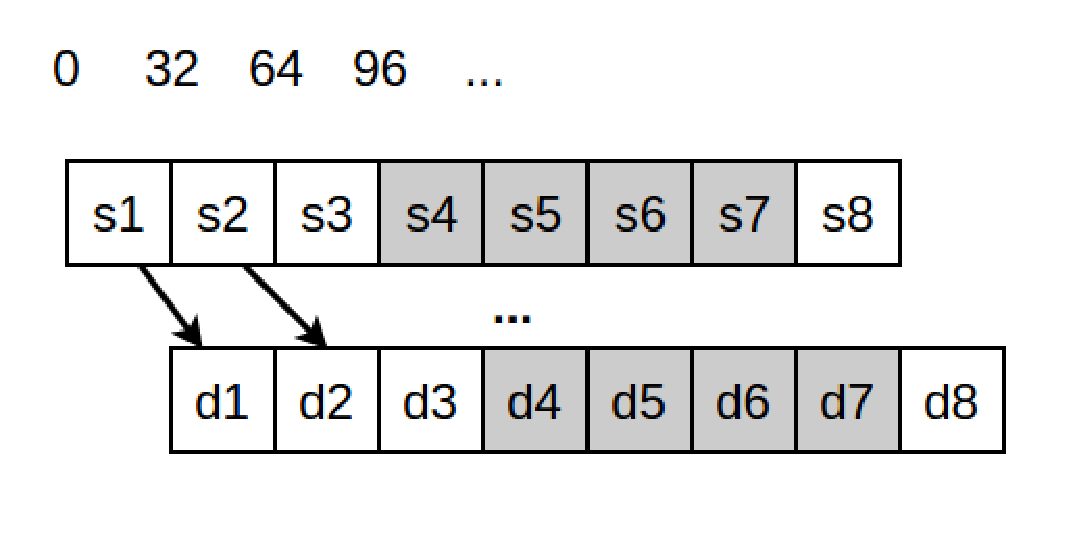
\includegraphics[width=10cm,height=6cm]{figures/chap03/offset32}
  \caption{32bit偏移下过程C算法举例}
  \label{fig:offset32}
\end{figure}

这里为了验证宽位访存指令的效果,进行了内存到内存的拷贝性能测试,测试结果如下:

\begin{center} \tablecaption{宽位访存指令优化效果测试 \label{tab:memcpy-performance-opt}} 
\tablefirsthead{
\rowcolor[gray]{0.8}
\multicolumn{1}{c}{\textbf{数据量大小}} &
\multicolumn{1}{c}{\textbf{优化前}} &
\multicolumn{1}{c}{\textbf{优化后}} \\ }
\tablehead{\multicolumn{3}{c}{
\small 表 \ref{tab:memcpy-performance-opt} (续) } \\
\rowcolor[gray]{0.8}
\multicolumn{1}{c}{\textbf{数据量大小}} &
\multicolumn{1}{c}{\textbf{优化前}} &
\multicolumn{1}{c}{\textbf{优化后}} \\ }
\tabletail{\bottomrule
\multicolumn{3}{c}{\small 接下页} \\}
\tablelasttail{\bottomrule}

%./svPerfGL -i ../../trisNormsColors-512.nc -w 1280 -h 1024 -2 -r -t 60 -s 3000000
\begin{supertabular}{p{6.cm}<{\centering}p{3.cm}<{\centering}m{6.cm}<{\centering}}
	4KB& 409MB/s& 819MB/s\\
	16KB& 564MB/s& 1260MB/s\\
	64KB& 313MB/s& 420MB/s\\
	256KB& 268MB/s& 399MB/s\\
	1MB& 246MB/s& 325MB/s\\
	4MB& 210MB/s& 227MB/s\\
	16MB& 201MB/s& MB/s\\
	64MB& 185MB/s& MB/s\\
	256MB& 178MB/s& 183MB/s\\
\end{supertabular}
\end{center}

\subsubsection{GPU拷贝效率的优化}

前面提到的CPU与GPU拷贝策略的优化是把数据放在GTT,然后让GPU来GTT访问数据,这样可能会加大GPU的负载,所以这里采用张凯的论文$<<$显存与内存间的数据传输通路优化$>>$\cite{gpu-cpu-data}里面提到采用GTT+DMA的这种非线性的优化方法,使用这种方法的原理就是GPU采用DMA的方式在不占用CPU的执行周期的情况下将GTT里面的内容快速的拷贝到显存中,这样GPU之后的访存时间就会减少,总体上减小了GPU的工作负载。

\begin{figure}[H] 
  \centering
  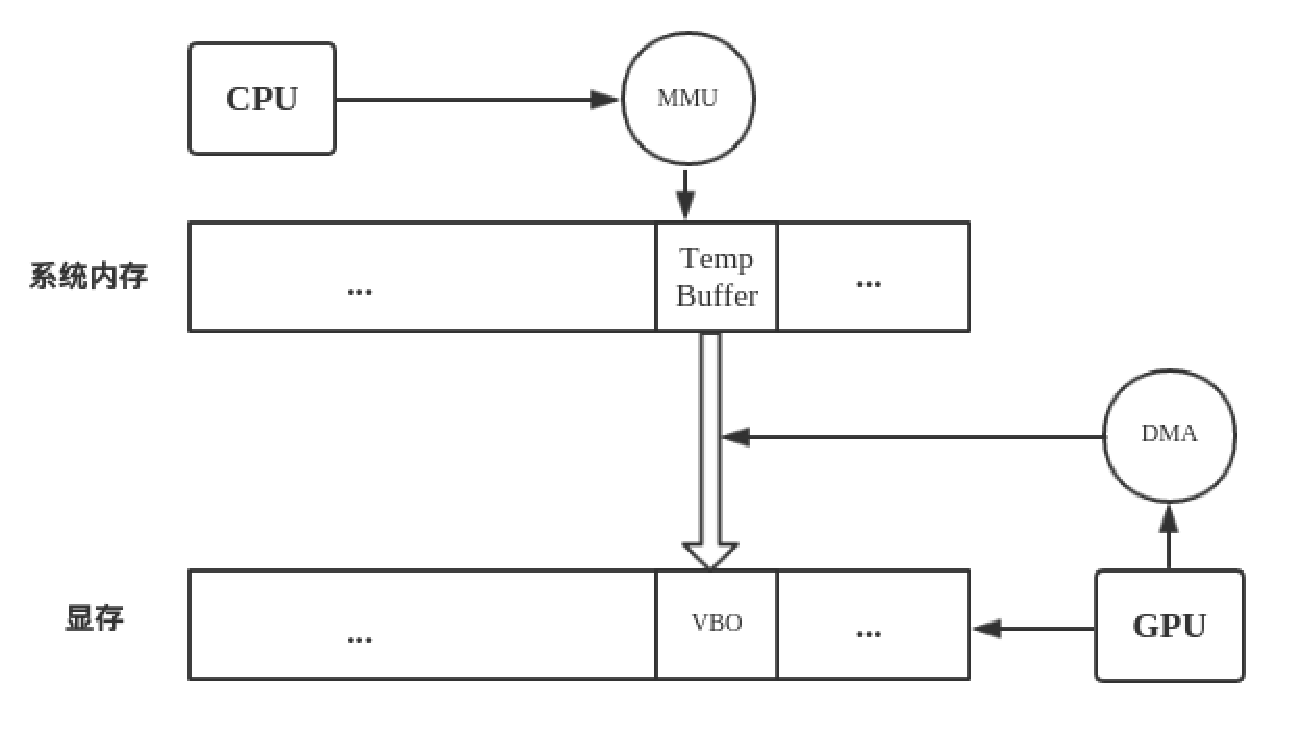
\includegraphics[width=12cm,height=8cm]{figures/chap03/gpu-dma}
  \caption{DMA方式下的Mesa3D库CPU与GPU访存策略}
  \label{fig:gpu-dma}
\end{figure}

改进的传输模式如图\ref{fig:gpu-dma},对比之前的实现(图\ref{fig:vbo-gtt}),虽然设计上更加复杂了一些,但是在龙芯平台上,PCI-E总线带宽较小,直接读写的速度非常慢, 这会导致即使在小数据量时直接读写的效率也比DMA方式的效率更低。


\section{Mesa3D的CPU端计算优化}

\subsection{研究背景}

\subsection{CPU端计算热点}

\subsection{CPU端优化技术}

\section{本章小结}


\chapter{测试与验证}

\section{测试与验证平台介绍}

\section{CPU与GPU负载平衡优化测试}

\section{内存与显存数据传输优化测试}

\section{本章小结}


\chapter{总结与展望}

\section{本文工作总结}

随着国际形势的日益复杂,计算机工业体系国产化的进程在加速推进,拥有完全自主知识产权的龙芯系列处理器作为计算机工业体系的核心基石,承担着更大的责任与期望。为了提高龙芯系列处理器的核心竞争力,更好更快的推进计算机工业体系的国产化的步伐,龙芯系列处理器的工作性能和图形使用体验就显得尤为重要。本文正是在这样的一个大背景下,展开对龙芯平台上的Mesa3D图形库的研究与优化工作。通过阅读Mesa3D、libdrm和radeon相关驱动源代码,深入分析龙芯平台Mesa3D库的实现原理与性能瓶颈,并针对性的进行优化。本文所做的主要工作如下:

\begin{itemize}
\item{} Mesa3D图形库CPU与GPU端负载分析与优化,由于龙芯平台的特殊性,现有Mesa3D图形库在CPU端的工作任务过多,导致CPU端执行负载较大成为性能的瓶颈,本文通过定位负载不平衡的原因,并提出有效的解决办法达到龙芯平台上Mesa3D图形库CPU与GPU的执行负载相对均衡,实现整体性能的提升。
\item{}	Mesa3D图形库内存到显存的数据传输的优化。本文分析了原有内存到显存的数据传输方法,并结合相关研究成果,改进了Mesa3D图形库内存到显存的数据传输策略,并使用宽位访存指令做出更进一步的优化,达到数据传输性能的提升。
\item{} Mesa3D图形库CPU端热点的优化。本文定位和分析了Mesa3D图形库在CPU端存在的计算热点,然后采用分支减少、循环简化以及编译优化等常用程序优化手段进行优化,提高了CPU端的执行性能。
\end{itemize}

\section{下一步研究方向}

本文的优化方法虽然在一定程度上能够提高龙芯平台Mesa3D图形库的性能,但是仍然存在一些问题需要未来的研究工作给予解决,未来主要工作主要有以下几个方面:

\begin{itemize}
\item{\textbf{龙芯平台的通用性}}: \\
本文所有研究和优化工作都是在龙芯3A-780E开发板上进行的,而龙芯系列处理器种类繁多,不同处理器平台搭载的GPU情况都不相同,特别是龙芯最新推出的3A2000和3B2000系列处理器,访存带宽有着很大的改进和提升,所以可能会造成一些性能瓶颈的不同。这就还需要具体环境具体分析然后修改和适配本文提出的几种优化方法。

\item{\textbf{VxWorks操作系统上的Mesa3D库移植与优化}}: \\
龙芯系列产品,除了桌面系列产品以外还包括嵌入式系列产品,目前龙芯嵌入式产品主要搭载着VxWorks操作系统,而目前该系统还没有支持Mesa3D,为了丰富嵌入式操作系统的图形表现能力,未来还需要在VxWorks操作系统上进行Mesa3D的移植和优化。

\item{\textbf{Mesa3D图形库最新版本的移植和优化}}: \\
本文优化的Mesa3D图形库是10.1.6版本,该版本是目前龙芯平台上的最新Mesa3D版本,而Mesa3D目前最新推出了11.2.0版本,在架构和性能上有一些改进,所以未来可以将最新的Mesa3D版本移植到龙芯平台并做出相关优化。

\end{itemize}




% 参考文献
\bibliographystyle{GBT7714-2005NLang-UTF8}
\bibliography{ref/refs}

% 附录
\begin{appendix}
%%% Local Variables: 
%%% mode: latex
%%% TeX-master: "../main"
%%% End: 

\chapter{OpenGL历史版本变更表 }
%\footnote{摘自OpenGL-维基百科}
\label{cha:OpenGL-History-Version}

%跨页表格
\begin{center} \tablecaption{OpenGL版本变更表 \label{tab:OpenGL-Version-History}} 
\tablefirsthead{
\rowcolor[gray]{0.8}
\multicolumn{1}{l}{\textbf{主要版本}} &
\multicolumn{1}{l}{\textbf{发布日期}} &
\multicolumn{1}{c}{\textbf{重要变更}} \\ }
\tablehead{\multicolumn{3}{c}{
\small 表 \ref{tab:OpenGL-Version-History} (续) } \\
\rowcolor[gray]{0.8}
\multicolumn{1}{l}{\textbf{主要版本}} &
\multicolumn{1}{l}{\textbf{发布日期}} &
\multicolumn{1}{c}{\textbf{重要变更}} \\ }
\tabletail{\bottomrule
\multicolumn{3}{c}{\small 接下页} \\}
\tablelasttail{\bottomrule}

\begin{supertabular}{p{2.cm}p{2.cm}p{11.cm}}
      1.1 & 1997.1 & \\
      1.2 & 1998.3 & \\
      1.2.1 & 1998.10 & \\
      1.3 & 2001.8 & \\
      1.4 & 2002.7 & \\
      1.5 & 2003.7 & \\
      2.0 & 2004.9 & \\
      2.1 & 2006.7 & \\
      3.0 & 2008.8 & \\
      3.1 & 2009.3 & \\
      3.2 & 2009.8 & \\
      3.3 & 2010.3 & \\
      4.0 & 2010.3 & \\
      4.1 & 2010.7 & \\
      4.2 & 2011.8 & 
支持的显卡: \\
& & Nvidia GeForce 400 series, Nvidia GeForce 500 series, Nvidia GeForce 600 series, ATI Radeon HD 5000 series, AMD Radeon HD 6000 Series, AMD Radeon HD 7000 Series \\
& & \tabitem 支持Shaders原子计数器和加载、存储、原子读-修改-写操作的单级纹理着色器。\\
& & \tabitem捕捉GPU-tessellated几何变换反馈的结果绘制的多个实例,使复杂的对象进行有效的重新定位和复制。\\
& & \tabitem支持修改任意子集的压缩纹理,而无需重新下载整个GPU的纹理,显著的性能改进。\\
& & \tabitem支持包装成一个单一的32位值显著降低内存存储和带宽的高效着色处理多个8位和16位值。\\
    %\toprule[1.5pt] 
      4.3 & 2012.8 & 支持的显卡: \\
& & NVIDIA GeForce400系列,NVIDIA GeForce500系列,NVIDIA GeForce600系列,NVIDIA GeForce700系列,ATI Radeon HD 5000系列,AMD Radeon HD6000系列,AMD Radeon HD7000系列,AMD Radeon HD8000系列 \\
& & \tabitem 围内充分利用GPU的并发计算着色器的图形管道 \\
& & \tabitem 暗器的存储缓冲器对象 \\
& & \tabitem 纹理参数查询 \\
& & \tabitem 作为标准功能的高质量的纹理压缩ETC2/EAC \\
& & \tabitem 完全兼容的OpenGL ES3.0的API \\
& & \tabitem 在应用程序开发过程中调试能力接收调试消息 \\
& & \tabitem 没有数据复制以不同的方式解释纹理的纹理意见 \\
& & \tabitem 增加了内存的安全性 \\
& & \tabitem 一个多应用的健壮性扩展 \\
      4.4 & 2013.7 & 支持的显卡: \\
& & DIA GeForce 400系列、NVIDIA GeForce 500系列、NVIDIA GeForce 600系列、NVIDIA GeForce 700系列,ATI Radeon HD 5000系列、AMD Radeon HD6000系列、AMD Radeon HD7000系列、AMD Radeon R9/R7 200系列 \\
& & \tabitem 缓冲器位置控制 \\
& & \tabitem 高效异步查询 \\
& & \tabitem 着色器可变布局 \\
& & \tabitem 高效多对象绑定 \\
& & \tabitem 精简化Direct3D应用的移植 \\
& & \tabitem 非绑定的纹理扩展 \\
& & \tabitem 稀疏纹理扩展 \\
      4.5 & 2014.8 & \\
\end{supertabular}
\end{center}

\chapter{Mesa3D历史版本变更表}
\label{cha:Mesa3D-History-Version}

\begin{center} \tablecaption{Mesa3D版本变更表(4.0之前版本不再支持) \label{tab:Mesa3D-Version-History}} 
\tablefirsthead{
\rowcolor[gray]{0.8}
\multicolumn{1}{l}{\textbf{主要版本}} &
\multicolumn{1}{l}{\textbf{发布日期}} &
\multicolumn{1}{c}{\textbf{支持OpenGL版本}} \\ }
\tablehead{\multicolumn{3}{c}{
\small 表 \ref{tab:OpenGL-Version-History} (续) } \\
\rowcolor[gray]{0.8}
\multicolumn{1}{l}{\textbf{主要版本}} &
\multicolumn{1}{l}{\textbf{发布日期}} &
\multicolumn{1}{c}{\textbf{支持OpenGL版本}} \\ }
\tabletail{\bottomrule
\multicolumn{3}{c}{\small 接下页} \\}
\tablelasttail{\bottomrule}

\begin{supertabular}{p{2.cm}p{2.cm}m{11.cm}}
      11.2 & 2016.3 & 4.2(Intel 3.3)\\
      11.1 & 2015.12 & 4.2(Intel 3.3)\\
      11.0 & 2015.9 & 4.2(Intel 3.3)\\
      10.6 & 2015.6 & 3.3\\
      10.5 & 2015.3 & 3.3\\
      10.4 & 2014.12 & 3.3\\
      10.3 & 2014.9 & 3.3\\
      10.2 & 2014.6 & 3.3\\
      10.1 & 2014.3 & 3.3\\
      10.0 & 2013.11 & 3.3\\
      9.0 & 2012.10 & 3.1\\
      8.0 & 2012.2 & 3.0\\
      7.0 & 2007.6 & 2.1\\
      6.0 & 2004.1 & 1.5\\
      5.0 & 2002.11 & 1.4\\
      4.0 & 2001.10 & 1.3\\
\end{supertabular}
\end{center}


\chapter{ATTR宏函数}
%\footnote{摘自OpenGL-维基百科}
\label{cha:attr}

\begin{lstlisting}
/**
 * This macro is used to implement all the glVertex, glColor, glTexCoord,
 * glVertexAttrib, etc functions.
 */
#define ATTR( A, N, T, V0, V1, V2, V3 )					\
do {									\
   struct vbo_exec_context *exec = &vbo_context(ctx)->exec;		\
									\
   if (unlikely(!(ctx->Driver.NeedFlush & FLUSH_UPDATE_CURRENT)))	\
      ctx->Driver.BeginVertices( ctx );					\
   									\
   if (unlikely(exec->vtx.active_sz[A] != N))				\
      vbo_exec_fixup_vertex(ctx, A, N);					\
   									\
   {									\
      GLfloat *dest = exec->vtx.attrptr[A];				\
      if (N>0) dest[0] = V0;						\
      if (N>1) dest[1] = V1;						\
      if (N>2) dest[2] = V2;						\
      if (N>3) dest[3] = V3;						\
      exec->vtx.attrtype[A] = T;                                        \
   }									\
									\
   if ((A) == 0) {							\
      /* This is a glVertex call */					\
      GLuint i;								\
									\
      for (i = 0; i < exec->vtx.vertex_size; i++)			\
	 exec->vtx.buffer_ptr[i] = exec->vtx.vertex[i];			\
									\
      exec->vtx.buffer_ptr += exec->vtx.vertex_size;			\    
									\
      /* Set FLUSH_STORED_VERTICES to indicate that there's now */	\
      /* something to draw (not just updating a color or texcoord).*/	\
      ctx->Driver.NeedFlush |= FLUSH_STORED_VERTICES;			\
									\
      if (++exec->vtx.vert_count >= exec->vtx.max_vert)			\
	 vbo_exec_vtx_wrap( exec );					\
   }									\
} while (0)
\end{lstlisting}



\end{appendix}

%%% 其他部分
\backmatter

% 致谢
%%% Local Variables:
%%% mode: latex
%%% TeX-master: "../main"
%%% End:

\begin{ack}
  衷心感谢我的导师胡伟武研究员对本人的精心指导。他们的言传身教将使...
\end{ack}


% 作者简介
\begin{resume}

\noindent
姓名:胡庆海  性别:男  出生日期:1991.10.18  籍贯:安徽\\

\noindent
2013.9 -- 现在      中国科学院计算技术研究所\quad微处理器研究中心\qquad硕士

\noindent
2009.9 -- 2013.7     中国科学技术大学\quad计算机科学与技术系\qquad本科\\

  \resumeitem{攻读硕士学位期间参加的科研项目} % 有就写,没有就删除
  \begin{enumerate}[{[}1{]}]
  \item 龙芯平台QT库优化, 2014年11月~2015年6月
  \item 龙芯平台Mesa库优化, 2015年9月~2016年2月 
  \end{enumerate}

  \resumeitem{攻读硕士学位期间的专利成果} % 有就写,没有就删除
  \begin{enumerate}[{[}1{]}]
  \item  一种模拟编译器实现C++函数动态调用的方法(在申)
  \item  一种基于SIMD的QT库基本图元绘制加速的方法(在申)
  \item  多核龙芯平台下实现共享内存式MapReduce计算框架(在申)
  \end{enumerate}

  \resumeitem{攻读硕士学位期间的获奖情况} % 有就写,没有就删除
  \begin{enumerate}[{[}1{]}]
  \item  2015年被评为中国科学院“三好学生”
  \end{enumerate}
\end{resume}


% 保证总页数为偶数。连续双面打印时,防止将两份论文的末页、首页打印在同一张纸上。
\cleardoublepage

\end{document}
